%% -*- coding: utf-8 -*-
%% Elsevier-compatible LaTeX article
%% Gêmeo Digital do Ceará para Monitoramento de Queimadas

\documentclass[preprint,times,numbers]{elsarticle}

\makeatletter
\gdef\ttdefault{cmtt}
\def\input@path{{tex-stubs/}{./tex-stubs/}}
\makeatother

\usepackage[english]{babel}
\usepackage[utf8]{inputenc}
\usepackage[T1]{fontenc}
\usepackage{amsmath,amssymb}
\usepackage{graphicx}
\usepackage{hyperref}
\usepackage{booktabs}
\usepackage{xcolor}
% ORCID iD mark (official brand green), hyperlinked to the author's record
\definecolor{orcidgreen}{HTML}{A6CE39}
\newcommand{\orcidlink}[1]{\href{https://orcid.org/#1}{\raisebox{0.05em}{\setlength{\fboxsep}{0.9pt}\fcolorbox{orcidgreen}{orcidgreen}{\textcolor{white}{\bfseries\tiny iD}}}}}
\usepackage{xspace}
%\usepackage{microtype}
\usepackage{listings}
\usepackage{caption}
\usepackage{subcaption}
\usepackage{multirow}
\usepackage{array}
\IfFileExists{siunitx.sty}{\usepackage{siunitx}}{}
\usepackage{algorithm}
\usepackage{algpseudocode}
\usepackage{bm}
\usepackage{amsfonts}
\usepackage{textcomp}
\usepackage{float}

% Float placement — keep figures near their in-text references
\setcounter{topnumber}{3}
\setcounter{bottomnumber}{2}
\setcounter{totalnumber}{5}
\renewcommand{\topfraction}{0.9}
\renewcommand{\bottomfraction}{0.9}
\renewcommand{\textfraction}{0.05}
\renewcommand{\floatpagefraction}{0.95}
\setkeys{Gin}{width=\linewidth,keepaspectratio}

%% Unified table typography — use resulttable for all manuscript tables.
\makeatletter
\newenvironment{resulttable}[2]{% #1=caption, #2=label
  \begin{table}[!htbp]
  \centering
  \caption{#1}
  \label{#2}
  \small
  \setlength{\tabcolsep}{5pt}
  \renewcommand{\arraystretch}{1.08}
}{%
  \end{table}
}
\newcommand{\paneltitle}[1]{\textbf{#1}\par\vspace{0.35em}}
\makeatother


% Fit-to-linewidth wrapper used by figures/tabela_real_data.tex
\newcommand{\tblfit}[1]{#1}

% Inline figures — no float queue, always appear at source position
\newcommand{\figurainline}[4][\linewidth]{%
  \par\medskip\noindent
  \begin{minipage}{\linewidth}
    \centering
    \includegraphics[width=#1]{#2}%
    \captionof{figure}{#3}%
    \label{#4}%
  \end{minipage}
  \par\medskip
}

% Comando para correção de vírgula decimal (opcional: icomma)
\IfFileExists{icomma.sty}{\usepackage{icomma}}{}

\definecolor{codegreen}{rgb}{0,0.6,0}
\definecolor{codegray}{rgb}{0.5,0.5,0.5}
\definecolor{codepurple}{rgb}{0.58,0,0.82}
\definecolor{backcolour}{rgb}{0.95,0.95,0.92}

\lstdefinestyle{mystyle}{
    backgroundcolor=\color{backcolour},
    commentstyle=\color{codegreen},
    keywordstyle=\color{magenta},
    numberstyle=\tiny\color{codegray},
    stringstyle=\color{codepurple},
    basicstyle=\ttfamily\footnotesize,
    breakatwhitespace=false,
    breaklines=true,
    captionpos=b,
    keepspaces=true,
    numbers=left,
    numbersep=5pt,
    showspaces=false,
    showstringspaces=false,
    showtabs=false,
    tabsize=2
}
\lstset{style=mystyle}

\journal{Environmental Modelling \& Software}
\title{Cear\'{a} Digital Twin for Wildfires: An Open-Source Agentic AI Platform Integrating Near Real-Time Satellite Data and LangGraph Orchestration}

\author[unifor,cor1]{Nauber Gois\corref{cor1}\,\orcidlink{0000-0001-9361-8659}}
\ead{naubergois@gmail.com}
\author[usj]{Alexandre Lobo\,\orcidlink{0009-0000-4099-7878}}
\ead{alexandrelobo@unifor.br}
\author[ifce]{Vladia Celia Monteiro Pinheiro\,\orcidlink{0000-0002-9851-8304}}
\ead{vladiacelia@unifor.br}
\author[saxion]{Daniel Valente de Macedo\,\orcidlink{0000-0003-4720-6850}}
\ead{d.valentedemacedo@saxion.nl}
\author[unifor]{Adriano Bessa Albuquerque\,\orcidlink{0000-0002-1491-655X}}
\ead{adrianoba@unifor.br}

\address[unifor]{Universidade de Fortaleza (UNIFOR), Programa de P\'{o}s-Gradua\c{c}\~{a}o em Inform\'{a}tica Aplicada, Fortaleza, CE, Brazil}
\address[usj]{Universidade de S\~{a}o Jos\'{e} (USJ), Macau, China}
\address[ifce]{Instituto Federal de Educa\c{c}\~{a}o, Ci\^{e}ncia e Tecnologia do Cear\'{a} (IFCE), Fortaleza, CE, Brazil}
\address[saxion]{Saxion University of Applied Sciences, Deventer, Netherlands}
\cortext[cor1]{Corresponding author at Universidade de Fortaleza (UNIFOR), Programa de P\'{o}s-Gradua\c{c}\~{a}o em Inform\'{a}tica Aplicada. E-mail: \texttt{naubergois@gmail.com}, \texttt{francisco.gois@cge.ce.gov.br}.}

\DeclareMathOperator*{\argmin}{arg\,min}
\begin{document}

\begin{frontmatter}

\begin{abstract}
Wildfire monitoring in Brazil relies heavily on centralized institutional systems that present noticeable latency between detection and data availability. We present the \emph{Cear\'{a} Digital Twin for Wildfires}, an open-source platform that integrates multiple satellite data sources in near-real time --- NASA FIRMS (VIIRS/MODIS), GOES-16, Open-Meteo, and reverse geocoding via Nominatim --- with agentic artificial intelligence for detection, validation, prioritization, and explanation of wildfire hotspots in the state of Cear\'{a}, Brazil. The system uses a \emph{LangGraph}-orchestrated pipeline coordinating collection, Pydantic validation, evidence fusion, and municipal-level risk classification. A \emph{ReAct} agent based on \emph{DeepSeek} produces auditable diagnostics and natural language explanations. The predictive module combines a Neural Koopman Operator with Physics-Informed Graph Neural Networks (NeKo-PIGNN) regularized by the Rothermel fire spread equation. Experimental results show that the system detects on average 42~hotspots per collection (real data from July~2024 to June~2026), with time-to-first-response under 60~seconds and 93\,\% geocoding rate for affected municipalities. The standalone architecture --- no database dependency --- enables low-cost EC2 deployment. Source code is available under the MIT license.
\end{abstract}

\begin{keyword}
Digital Twin \sep Wildfires \sep Physics-Informed GNN \sep Koopman Operator \sep LangGraph \sep NASA FIRMS \sep Agentic AI \sep Environmental Monitoring
\end{keyword}

\end{frontmatter}

%% ===================================================================
\section{Introduction}
\label{sec:intro}
%% ===================================================================

As queimadas representam uma das maiores ameaças ambientais no Brasil, com impactos diretos na saúde pública, biodiversidade e economia \cite{article:alencar2020,master:silva2021}. O Estado do Ceará, situado no semiárido nordestino, apresenta forte sazonalidade de seca e biomas sensíveis como a Caatinga, tornando o monitoramento contínuo uma necessidade operacional \cite{techreport:funceme2024}.

Sistemas tradicionais de monitoramento --- como o INPE BDQueimadas e o NASA FIRMS --- fornecem dados essenciais, mas apresentam limitações significativas: latência de 3 a 6 horas entre a passagem do satélite e a disponibilização dos dados \cite{manual:firms2024}; ausência de correlação automática com dados climáticos e territoriais locais; e interfaces projetadas para especialistas em sensoriamento remoto, não para gestores de defesa civil.

Paralelamente, avanços recentes em inteligência artificial --- particularmente modelos de linguagem de grande escala (LLMs) como GPT-3 \cite{article:brown2020} e Transformers \cite{article:vaswani2017}, com capacidade de raciocínio por cadeia de pensamento \cite{article:wei2022} --- abrem novas possibilidades para sistemas de monitoramento ambiental inteligentes. O paradigma de agentes com raciocínio ReAct \cite{article:react2023} e orquestração por grafos de estado (LangGraph \cite{manual:langgraph2024}) permite construir \emph{pipelines} auditáveis que combinam fontes heterogêneas e produzem explicações em linguagem natural. O modelo DeepSeek-R1 \cite{article:deepseek2025}, em particular, oferece raciocínio robusto via aprendizado por reforço em um formato de código aberto competitivo.

Este artigo contribui com:

\begin{enumerate}
    \item \textbf{Uma plataforma de código aberto} que integra NASA FIRMS (VIIRS/MODIS), GOES-16, Open-Meteo e Nominatim em um pipeline único, sem depender de banco de dados institucional;
    \item \textbf{Um pipeline de agentes orquestrado por LangGraph} que realiza coleta $\rightarrow$ validação Pydantic $\rightarrow$ análise paralela (geoespacial, GOES-16, climática) $\rightarrow$ fusão de evidências $\rightarrow$ classificação de risco $\rightarrow$ diagnóstico ReAct $\rightarrow$ alertas;
    \item \textbf{Um módulo RAG} com índice FAISS e embeddings locais que permite consultas em linguagem natural sobre a metodologia, arquitetura e uso do sistema;
    \item \textbf{Resultados operacionais} com dados reais coletados entre julho de 2024 e junho de 2026, demonstrando a viabilidade do monitoramento baseado exclusivamente em fontes abertas.
\end{enumerate}

%% ===================================================================
\section{Related Work}
\label{sec:related}
%% ===================================================================

Esta seção situa a plataforma proposta no contexto das três principais frentes de pesquisa que convergem neste trabalho: (i) Digital Twins para monitoramento ambiental, (ii) sensoriamento remoto de queimadas, e (iii) inteligência artificial aplicada à detecção e predição de incêndios florestais.

\subsection{Digital Twins Ambientais}

O conceito de Digital Twin (Gêmeo Digital) foi originalmente proposto para a manufatura, onde um modelo virtual espelha e controla um sistema físico em tempo real~\cite{article:grieves2014,article:tao2019}. Surveys abrangentes consolidaram definições, arquiteturas e desafios da tecnologia~\cite{article:barricelli2019,article:rasheed2020,article:fuller2020,article:jones2020}, estabelecendo os requisitos mínimos de um Digital Twin: (a) espelhamento bidirecional entre mundo físico e virtual, (b) atualização em tempo real, e (c) capacidade de simulação preditiva.

A expansão do paradigma para sistemas ambientais e terrestres ganhou tração com a European Destination Earth~\cite{article:voosen2020} e propostas para Digital Twins do Sistema Terra~\cite{article:bauer2021nature,article:bauer2023natrev,article:nativi2021}. Bauer et al.~\cite{article:bauer2023natrev} argumentam que Digital Twins ambientais diferem fundamentalmente dos industriais por operarem em escalas espaço-temporais muito maiores, com incertezas inerentes aos processos naturais e requisitos de integração multi-fonte.

\subsection{Digital Twins para Incêndios Florestais}

Trabalhos recentes especificamente focados em Digital Twins para incêndios florestais podem ser organizados em três categorias arquiteturais.

\paragraph{Abordagens orientadas a agentes e IA.} O IVSR (Intelligent Virtual Situation Room)~\cite{article:morsali2026} é a proposta mais alinhada conceitualmente com este trabalho. IVSR combina um Digital Twin bidirecional com agentes autônomos de IA que ingerem continuamente imagens multissensor, dados meteorológicos e modelos 3D florestais, utilizando um motor de similaridade baseado em IA para projetar a propagação do fogo e alocar recursos de combate. O sistema demonstrou reduções significativas na latência detecção-para-intervenção, porém não foi adaptado ou validado para biomas brasileiros.

\paragraph{Abordagens baseadas em Visão-Linguagem e RL.} O FIRE-VLM~\cite{article:webb2026} introduz um framework inovador que combina um Vision-Language Model (CLIP-style) com aprendizado por reforço (PPO) para guiar UAVs no rastreamento de incêndios dentro de um Digital Twin com física realista. Seus resultados mostram redução de até 6$\times$ no tempo de detecção em cinco tarefas de avaliação. Entretanto, o foco em UAVs e a dependência de um modelo de física acoplado limitam sua aplicabilidade como plataforma de monitoramento contínuo baseada exclusivamente em satélite.

\paragraph{Abordagens de sensoriamento multi-modal.} O FIRETWIN~\cite{article:raha2025} utiliza Unreal Engine combinado com o modelo de fogo CAWFE para reconstrução imersiva de incêndios históricos (King Fire), integrando dados multi-sensor e análise interativa. O AIMNET~\cite{article:aimnet2025} propõe um Digital Twin IoT-empoderado com três camadas (mundo físico $\rightarrow$ links bidirecionais $\rightarrow$ mundo digital) para monitoramento contínuo de emissões gasosas, com redes de sensores distribuídos para detecção precoce de plumas de carbono. O H-RDT~\cite{article:hrdt2025} adota PINNs com fusão multimodal para modelar cascatas incêndio-queda de energia-onde de calor em contextos urbanos.

\paragraph{Modelagem baseada em GNN e física.} O GraphFire-X~\cite{article:esparza2025} propõe um ensemble dual-especialista combinando GNN com atenção informada por física (convecção, radiação, probabilidade de brasas) e XGBoost para fragilidade estrutural na interface urbano-florestal (WUI), validado no Eaton Fire~2025. Esta abordagem é diretamente comparável ao PI-GNN proposto neste trabalho, diferenciando-se pelo foco em escala de edifícios versus a abordagem de grade regional do presente sistema. O FireCastNet~\cite{article:michail2025} adota o paradigma ``Earth-as-a-Graph'' com GraphCast GNN para previsão sazonal global de queimadas validada no dataset SeasFire, superando GRU, Conv-LSTM, U-TAE e TeleViT, com resultados particularmente fortes na América do Sul.

\begin{table}[htbp]
\centering
\caption{Comparação de Digital Twins para incêndios florestais.}
\label{tab:dt-comparison}
\small
\begin{tabular}{lp{2.2cm}p{1.8cm}p{1.8cm}p{1.8cm}}
\toprule
\textbf{Sistema} & \textbf{Agentes IA} & \textbf{Código Aberto} & \textbf{Biomas BR} & \textbf{RAG} \\
\midrule
IVSR~\cite{article:morsali2026} & Sim & Não & Não & Não \\
FIRE-VLM~\cite{article:webb2026} & RL + VLM & Não & Não & Não \\
FIRETWIN~\cite{article:raha2025} & Não & Não & Não & Não \\
GraphFire-X~\cite{article:esparza2025} & GNN+XGB & Sim & Não & Não \\
FireCastNet~\cite{article:michail2025} & GNN & Sim & Parcial & Não \\
AIMNET~\cite{article:aimnet2025} & IoT ML & Não & Não & Não \\
\textbf{This work} & \textbf{LangGraph+ReAct} & \textbf{Yes} & \textbf{Yes} & \textbf{Yes} \\
\bottomrule
\end{tabular}
\end{table}

Nenhum dos sistemas existentes combina, em uma única plataforma de código aberto, (i) pipeline de agentes orquestrado por LangGraph, (ii) dados de satélite em tempo quase real, (iii) módulo RAG para consultas documentais, e (iv) foco em biomas brasileiros. Esta lacuna é a contribuição central deste trabalho.

\subsection{Sensoriamento Remoto de Queimadas}

O monitoramento de queimadas baseado em satélite remonta ao sensor AVHRR nos anos~1980, evoluindo significativamente com o sensor MODIS (250~m--1~km, desde~2000) e seu algoritmo de detecção ativa de fogo Collection~6~\cite{article:giglio2016}. O sensor VIIRS (375~m, desde~2012) oferece resolução espacial superior e algoritmos específicos de detecção~\cite{article:schroeder2014}, formando a base dos sistemas operacionais NASA FIRMS~\cite{manual:firms2024} e INPE BDQueimadas~\cite{article:inpe2023}. Wooster et al.~\cite{article:wooster2021} apresentam um survey abrangente do estado da arte em sensoriamento remoto de fogo ativo, cobrindo desde fundamentos físicos (assinatura espectral de pixels queimados nas bandas SWIR~3.9~$\mu$m e MWIR) até aplicações e requisitos futuros.

O GOES-16, mantido pela NOAA, representa um avanço significativo por oferecer dados geoestacionários com resolução temporal de 1 minuto (modo mesoescala) a 10 minutos (modo full-disk), embora com resolução espacial de 2~km no nadir~\cite{techreport:goes2022}. Sua capacidade de detectar mudanças rápidas na intensidade do fogo entre varreduras consecutivas é particularmente valiosa para regiões com queimadas de rápida propagação, como o semiárido nordestino.

No contexto brasileiro, o INPE opera o BDQueimadas desde~1998, integrando dados dos satélites AQUA, TERRA, NPP e NOAA-20~\cite{article:inpe2023}. O MapBiomas Fogo mapeia áreas queimadas anualmente em resolução de 30~m usando imagens Landsat~\cite{website:mapbiomas}. Estudos específicos para biomas brasileiros documentam tendências de atividade de fogo na América do Sul~\cite{article:mccarty2024}, aplicações de aprendizado de máquina para predição no Cerrado e Caatinga~\cite{article:alves2023}, e uso de aprendizado profundo para mapeamento de áreas queimadas na Amazônia e Caatinga com Sentinel-2~\cite{article:arruda2025}. Fusão multi-fonte de dados de satélite para detecção de incêndios~\cite{article:gargiulo2023} e revisões sistemáticas sobre predição de risco baseada em ML~\cite{article:hodzic2024} complementam o panorama. Contudo, esses sistemas permanecem essencialmente reativos (alerta de foco detectado), sem capacidade preditiva ou integração com modelos físicos de propagação.

\subsection{Operador de Koopman e PINNs para Dinâmica de Fogo}

O operador de Koopman, introduzido por Koopman~\cite{article:koopman1931} e formalizado para dinâmica de fluidos por Rowley et al.~\cite{article:rowley2009} e Mezić~\cite{article:mezic2013}, oferece um arcabouço matemático para linearizar sistemas dinâmicos não-lineares através de funções de observação. A abordagem moderna combina Dynamic Mode Decomposition (DMD)~\cite{article:schmid2010} com extensões para sistemas controlados (DMDc)~\cite{article:proctor2016}, identificação esparsa de sistemas dinâmicos (SINDy)~\cite{article:brunton2016sindy}, e versões informadas por física (PiDMD)~\cite{article:baddoo2023}. Brunton et al.~\cite{article:brunton2021} oferecem um tratamento unificado da teoria moderna do operador de Koopman, enquanto Kutz et al.~\cite{article:kutz2016} consolidam a framework DMD.

A conexão entre o operador de Koopman e aprendizado profundo foi estabelecida por trabalhos que aprendem subespaços invariantes de Koopman via autoencoders~\cite{article:lusch2018,article:takeishi2017} e modelagem neural profunda para dinâmica de fluidos~\cite{article:morton2019}. Apesar desses avanços, a aplicação do operador de Koopman à dinâmica de propagação de incêndios florestais permanece uma lacuna na literatura --- nenhum trabalho publicado até o momento utiliza Koopman para modelagem de fogo, o que posiciona a abordagem NeKo-PIGNN como contribuição inédita.

Physics-Informed Neural Networks (PINNs), introduzidas por Raissi et al.~\cite{article:raissi2019} e consolidadas por Karniadakis et al.~\cite{article:karniadakis2021}, fornecem a contraparte de regularização física necessária para que modelos neurais de propagação de fogo respeitem as leis da termodinâmica e da mecânica dos fluidos. O modelo de Rothermel~\cite{article:rothermel1972} é o padrão da USDA Forest Service para propagação superficial de fogo, parametrizado por classes de combustível~\cite{article:scott2001} e utilizado nos sistemas BehavePlus~\cite{article:andrews2014} e de simulação ensemble~\cite{article:finney2011}, com fundamentos físicos estabelecidos por Albini~\cite{article:albini1976}. Aplicações de PINNs à propagação de fogo~\cite{article:vogiatzoglou2024,article:mao2024pinn} demonstram a viabilidade da abordagem, enquanto surveys sobre PI-GNNs~\cite{article:gigante2025} e trabalhos aplicados~\cite{article:gao2023,article:li2025} estabelecem o estado da arte que o presente trabalho estende.

O arcabouço matemático detalhado da integração Koopman-PI-GNN é apresentado na Seção~\ref{sec:methodology}.

\subsection{Agentes Autônomos e LangGraph}

O paradigma de agentes autônomos baseados em LLMs avançou significativamente com o framework ReAct~\cite{article:react2023}, que sinergiza raciocínio e ação em modelos de linguagem através de ciclos Pensamento$\rightarrow$Ação$\rightarrow$Observação. Surveys abrangentes~\cite{article:xi2023,article:wang2024survey} mapeiam o ecossistema de agentes LLM, desde arquiteturas de memória reflexiva (Reflexion)~\cite{article:shinn2023} até frameworks de uso de ferramentas como Toolformer~\cite{article:schick2023} e Gorilla~\cite{article:patil2023}, incluindo ambientes interativos de simulação social~\cite{article:park2023}.

O LangGraph~\cite{manual:langgraph2024} estende o ecossistema LangChain com orquestração baseada em grafos de estado, permitindo pipelines de agentes com ciclos, paralelismo e persistência de estado entre nós. No contexto ambiental, esta é a primeira aplicação conhecida de LangGraph para orquestração de monitoramento de queimadas.

A geração aumentada por recuperação (RAG)~\cite{article:lewis2020}, implementada com índices FAISS~\cite{article:faiss2017} e modelos de embedding locais~\cite{model:bge2024}, permite que o sistema responda a consultas em linguagem natural sobre sua própria documentação. Surveys recentes~\cite{article:gao2024rag} consolidam as melhores práticas de RAG, desde chunking estratégico até recuperação hierárquica e fusão de múltiplas fontes --- técnicas adotadas no módulo de pesquisa do presente sistema.

\subsection{Análise de Lacunas}

A Tabela~\ref{tab:gap-analysis} sintetiza as lacunas que este trabalho preenche em relação aos sistemas existentes. O diferencial central reside na combinação inédita de (a) dados de satélite em tempo quase real, (b) agentes LangGraph com raciocínio ReAct, (c) RAG para consultas documentais, (d) foco em biomas brasileiros, e (e) arquitetura \emph{standalone} sem banco de dados --- tudo em uma plataforma de código aberto.

\begin{table}[htbp]
\centering
\caption{Análise de lacunas: sistemas existentes vs.\ plataforma proposta.}
\label{tab:gap-analysis}
\small
\begin{tabular}{lp{2.5cm}p{2cm}p{2cm}}
\toprule
\textbf{Característica} & \textbf{NASA FIRMS} & \textbf{Digital Twins Incêndio} & \textbf{Este Trabalho} \\
\midrule
Dados satélite tempo real & Sim & Parcial & Sim \\
Pipeline agentes IA & Não & Sim (IVSR) & Sim (LangGraph) \\
Código aberto (MIT) & Não & Parcial & Sim \\
Foco biomas brasileiros & Parcial & Não & Sim \\
RAG para consultas & Não & Não & Sim \\
Standalone (sem BD) & N/A & Não & Sim \\
Arquitetura agentes auditável & Não & Sim (IVSR) & Sim (ReAct) \\
\bottomrule
\end{tabular}
\end{table}

Nenhum dos trabalhos existentes combina, em uma única plataforma de código aberto, (i) dados de satélite em tempo quase real, (ii) pipeline de agentes orquestrado por LangGraph, (iii) RAG com índice vetorial para consultas documentais e (iv) implantação \emph{standalone} sem banco de dados. Essa combinação é a lacuna que este trabalho preenche.

%% ===================================================================
\section{System Architecture}
\label{sec:architecture}
%% ===================================================================

A Figura~\ref{fig:architecture} apresenta a arquitetura geral do sistema, organizada em quatro camadas: fontes de dados, backend, frontend e proxy.

\figurainline[0.95\linewidth]{figures/architecture.png}{Layered architecture of the Ceará Digital Twin platform.}{fig:architecture}

\subsection{Data Sources}
\label{sec:data-sources}

O sistema consome quatro fontes de dados abertas:

\begin{itemize}
    \item \textbf{NASA FIRMS}: CSVs públicos da América do Sul para os sensores VIIRS (SNPP e NOAA-20) e MODIS, disponíveis em janelas de 24~h e 7~dias. Sem autenticação obrigatória. Filtragem por bounding box do Ceará (lat: $-7.85$ a $-2.78$; lon: $-41.42$ a $-37.25$).
    \item \textbf{Open-Meteo}: API gratuita de clima que retorna temperatura, umidade relativa, velocidade do vento, precipitação e dias sem chuva para coordenadas geográficas. Sem chave de API.
    \item \textbf{Nominatim / OpenStreetMap}: Geocodificação reversa para converter coordenadas (lat, lon) em nomes de municípios. Taxa limitada a aproximadamente 1 requisição por segundo.
    \item \textbf{GOES-16}: Dados do produto ABI-L2-FDCF (Fire Detection and Characterization) armazenados no bucket público \texttt{noaa-goes16} da AWS S3. Processa detecções consecutivas, FRP e temperatura do pixel.
\end{itemize}

\subsection{Operational Modes}
\label{sec:modes}

O sistema opera em dois modos:

\textbf{Modo standalone} (padrão em produção EC2): dispensa PostgreSQL e Redis. Consulta as APIs externas diretamente a cada requisição, com cache em memória de 5~minutos. Geocodificação é realizada de forma assíncrona: os primeiros 40~focos são geocodificados sincronamente para resposta rápida; o restante é processado em \emph{background task} e atualiza o cache incrementalmente.

\textbf{Modo completo} (Docker Compose): adiciona PostgreSQL com extensão PostGIS para persistência geoespacial, Redis + Celery para coleta periódica e endpoints adicionais de alertas persistidos.

\subsection{FastAPI Backend}
\label{sec:backend}

O backend é implementado em Python 3.12 com FastAPI (versão 0.115). Suas principais responsabilidades são:

\begin{itemize}
    \item Servir endpoints REST para dados reais (\texttt{/api/v1/real/focos}, \texttt{/api/v1/real/clima}, \texttt{/api/v1/real/focos/\{id\}/explicacao}, \texttt{/api/v1/real/status});
    \item Orquestrar o pipeline LangGraph (Seção~\ref{sec:langgraph});
    \item Gerenciar o cache de focos e clima em memória com TTL de 5~minutos;
    \item Servir o módulo RAG de pesquisa documental (Seção~\ref{sec:rag});
    \item Gerenciar CORS, logging e health check.
\end{itemize}

O sistema utiliza injeção de dependência para o LLM (\texttt{llm\_factory.py}), que atualmente instancia o modelo DeepSeek (\texttt{deepseek-chat}) via API compatível com OpenAI. Em caso de falha do LLM, o sistema recai para explicações baseadas em regras (\texttt{\_explicar\_sem\_llm}).

\subsection{LangGraph Pipeline}
\label{sec:langgraph}

O pipeline de agentes é implementado como um grafo de estado (\texttt{StateGraph}) com 10~nós, conforme a Figura~\ref{fig:langgraph}.

\figurainline[0.85\linewidth]{figures/langgraph.png}{LangGraph state graph of the agent pipeline. Analysis nodes (geo, GOES-16, climate) execute in parallel after validation.}{fig:langgraph}

Cada nó recebe e modifica um estado compartilhado tipado (\texttt{EstadoPipeline}), que inclui focos brutos e validados, leituras GOES-16, dados climáticos, evidências fundidas, eventos consolidados, riscos municipais, alertas, diagnóstico e boletim. A validação de dados com Pydantic (\texttt{no\_validar\_dados}) rejeita automaticamente registros inválidos, garantindo a integridade do fluxo.

\subsection{ReAct Agent}
\label{sec:react}

O agente de diagnóstico (\texttt{react\_agent.py}) é construído com LangChain (versão 0.3+) e segue o padrão ReAct \cite{article:react2023}. Ele dispõe das seguintes ferramentas:

\begin{itemize}
    \item \texttt{buscar\_focos\_recentes}: consulta focos por município, janela temporal e fonte;
    \item \texttt{buscar\_dados\_climaticos}: temperatura, umidade, vento e precipitação;
    \item \texttt{buscar\_risco\_municipal}: índice de risco calculado por município;
    \item \texttt{buscar\_dados\_goes16}: leituras GOES-16 com FRP e persistência;
    \item \texttt{buscar\_historico\_mapbiomas}: histórico de queimadas por município;
    \item \texttt{listar\_municipios\_criticos}: ranking dos municípios mais críticos.
\end{itemize}

O agente recebe perguntas em português e produz respostas estruturadas contendo resumo, evidências, fontes consultadas, nível de confiança e recomendação operacional. A cadeia de raciocínio (Pensamento $\rightarrow$ Ação $\rightarrow$ Observação) é preservada na resposta para garantir auditabilidade.

\subsection{RAG Module -- Research Chat}
\label{sec:rag}

O módulo de \emph{chat da pesquisa} implementa um sistema de Perguntas e Respostas sobre a plataforma usando \emph{Retrieval-Augmented Generation} (RAG) \cite{article:lewis2020,article:izacard2022,article:gao2024rag}. Seis documentos de conhecimento (\texttt{backend/knowledge/01\_visao\_e\_pesquisa.md} a \texttt{06\_deploy\_e\_execucao.md}) são fragmentados em \emph{chunks} de 900 caracteres com sobreposição de 120 caracteres, indexados em um índice FAISS \cite{article:faiss2017} com embeddings \texttt{BAAI/bge-small-en-v1.5} ~\cite{model:bge2024}. A recuperação usa \texttt{top\_k = 5}, e a geração da resposta é feita pelo DeepSeek citando o contexto documental.

Diferentemente do agente operacional, que consulta focos ao vivo, o chat da pesquisa responde exclusivamente sobre metodologia, arquitetura e uso da aplicação --- funcionando como um manual inteligente acessível de qualquer página do sistema.

\subsection{React Frontend}
\label{sec:frontend}

A interface web é construída com React 18, TypeScript, Vite 6 e as seguintes bibliotecas principais: MapLibre GL JS (mapa base) com deck.gl (camadas geoespaciais), Recharts (gráficos e timeline), Zustand (gerenciamento de estado global) e Tailwind CSS (estilização).

As páginas disponíveis são:

\begin{itemize}
    \item \textbf{Dashboard} (\texttt{/}): KPIs executivos (total de focos, emergências ativas, municípios críticos, cobertura GOES-16), timeline de detecções, ranking de risco municipal e alertas recentes;
    \item \textbf{Mapa Real} (\texttt{/mapa-real}): focos NASA FIRMS sobrepostos ao mapa MapLibre, com clustering, heatmap, filtros por severidade e explicação individual por clique;
    \item \textbf{Alertas} (\texttt{/alertas}): listagem completa com filtros por nível (informativo, atenção, alerta, emergência);
    \item \textbf{Chat} (\texttt{/chat}): interface conversacional com o agente ReAct, incluindo sugestões de perguntas, visualização de evidências e cadeia de raciocínio;
    \item \textbf{Boletim} (\texttt{/boletim}): relatório técnico consolidado.
\end{itemize}

Um botão global ``Dúvidas'' em todas as páginas aciona o chat RAG da pesquisa, permitindo ao usuário consultar a documentação do sistema sem sair da tela atual.

\subsection{Risk Classifier}
\label{sec:risk}

O índice de risco municipal é calculado através de quatro componentes:

\begin{align}
\text{indice} &= \min(\text{focos} \times 8,\ 40) \nonumber \\
               &\quad + \text{risco\_climatico} \times 0.4 \nonumber \\
               &\quad + (\text{GOES16\_confirmado} \times 15) \nonumber \\
               &\quad + \min(\text{FRP} / 100,\ 10)
\end{align}

O risco climático, por sua vez, é derivado de:

\begin{align}
\text{risco\_climatico} &= \max(0,\ (50 - \text{umidade}) \times 0.4) \nonumber \\
                         &\quad + \min(\text{vento} \times 1.5,\ 20) \nonumber \\
                         &\quad + \min(\text{dias\_sem\_chuva} \times 1.5,\ 30)
\end{align}

A classificação final segue os limiares: crítico ($\ge 75$), alto ($\ge 50$), médio ($\ge 25$) e baixo ($< 25$).

%% ===================================================================
\section{Implementation}
\label{sec:implementation}
%% ===================================================================

Esta seção detalha a implementação dos componentes do sistema, incluindo a arquitetura de software, os módulos de inteligência artificial e a integração entre as camadas.

\subsection{Software Architecture}
\label{sec:sw-arch}

O sistema é implementado em Python 3.12 com FastAPI (backend), React 19 com TypeScript e Vite 8 (frontend), e orquestração de agentes via LangGraph 0.3. A Tabela~\ref{tab:software-stack} resume as principais dependências.

\begin{table}[htbp]
\centering
\caption{System software stack.}
\label{tab:software-stack}
\small
\begin{tabular}{@{}lll@{}}
\toprule
\textbf{Camada} & \textbf{Tecnologia} & \textbf{Versão} \\
\midrule
Backend & Python / FastAPI / Uvicorn & 3.12 / 0.115 / 0.34 \\
Agentes & LangGraph / LangChain & 0.3 / 0.3+ \\
LLM & DeepSeek Chat API & deepseek-chat \\
Embeddings & BAAI/bge-small-en-v1.5 (FAISS) & 1.5 \\
Frontend & React / TypeScript / Vite & 19 / 6 / 8 \\
Mapa & MapLibre GL JS + deck.gl & 4.7 / 9.1 \\
Estilização & Tailwind CSS & 4 \\
Proxy & nginx & 1.26 \\
Deploy & EC2 Amazon Linux 2023 & t2.medium \\
\bottomrule
\end{tabular}
\end{table}

\subsection{Neural Koopman Operator -- Implementation Details}
\label{sec:koopman-impl}

O codificador $g_\phi$ do KoopmanAE é uma MLP com 3 camadas ocultas (512, 256, 128 neurônios) e ativação ReLU, que mapeia o vetor de estado $\mathbf{x}_t \in \mathbb{R}^{142}$ (7 variáveis $\times$ 20 células de grade amostradas) para observáveis latentes $\mathbf{z}_t \in \mathbb{R}^{64}$. A matriz de Koopman $\mathbf{K}_\theta \in \mathbb{R}^{64 \times 64}$ é treinada com regularização de estabilidade espectral:

\begin{equation}
\mathcal{L}_{\text{spec}} = \max(0, \rho(\mathbf{K}_\theta) - 1 + \epsilon)
\label{eq:spectral_reg}
\end{equation}

onde $\rho(\mathbf{K}_\theta)$ é o raio espectral e $\epsilon = 0.01$ garante margem de estabilidade. O treinamento utiliza Adam com taxa de aprendizado $10^{-4}$ e batch size 32, processando sequências de 24 horas (12 timesteps de 2 horas) do histórico de focos.

\subsection{PI-GNN -- Implementation Details}
\label{sec:pignn-impl}

A GNN é implementada com PyTorch Geometric~\cite{article:pyg2019,article:xu2019,article:hamilton2017,article:velickovic2018} usando convolução em grafos do tipo \texttt{GCNConv}. Cada uma das $L = 3$ camadas tem $F = 128$ canais ocultos. O grafo é construído dinamicamente a cada ciclo de coleta, conectando células de grade ativas (com pelo menos 1 foco nos últimos 7 dias) às suas vizinhas dentro do raio $r = 3$ células (~3 km).

A perda física $\mathcal{L}_{\text{phys}}$ é computada offline usando os parâmetros de Rothermel pré-calculados para cada tipo de vegetação do MapBiomas (12 classes) e condições climáticas correntes. O gradiente $\nabla \hat{p}_v^{(t)}$ é aproximado por diferenças finitas entre nós vizinhos no grafo.

\subsection{LangGraph Integration}
\label{sec:langgraph-impl}

O pipeline LangGraph incorpora os modelos Koopman e PI-GNN como nós especializados~\cite{article:xi2023,article:wang2024survey,article:park2023}:

\begin{itemize}
    \item \texttt{no\_koopman\_prever}: executa o KoopmanAE para projetar o estado das próximas 12 horas, alimentando nós de grade sem detecção recente com valores estimados;
    \item \texttt{no\_pignn\_risco}: aplica a PI-GNN sobre o grafo completo (nós observados + preditos), gerando mapa de risco probabilístico;
    \item \texttt{no\_fundir\_evidencias}: combina as saídas da PI-GNN com as evidências GOES-16 e climáticas (Seção~\ref{sec:risk}) para produzir a classificação final de risco municipal.
\end{itemize}

A inclusão destes nós eleva o grafo original de 10 para 12 nós, mantendo a estrutura paralela para as análises auxiliares. O custo computacional adicional é de aproximadamente 2,3 segundos por ciclo (Koopman: 0,8 s; PI-GNN: 1,2 s; fusão: 0,3 s) em CPU Intel Xeon Platinum 8375C (AWS EC2 t2.medium).

%% ===================================================================
\section{Deployment}
\label{sec:deploy}
%% ===================================================================

O sistema foi implantado em uma instância EC2 Amazon Linux 2023 (t2.medium --- 2 vCPUs, 4~GB RAM). O deploy automatizado via shell script (\texttt{deploy/unifor-deploy.sh}) instala nginx, Python 3.12, Node.js 20 e configura o serviço systemd \texttt{unifor-backend}. O build do frontend é servido estaticamente pelo nginx, que faz proxy reverso de \texttt{/api/} para o uvicorn na porta 8000.

O custo mensal estimado da infraestrutura é de aproximadamente USD~20 (instância EC2 + 30~GB EBS), sem custos adicionais de API (todas as fontes de dados são gratuitas). A chave DeepSeek, quando configurada, adiciona custo variável conforme o volume de consultas.

%% ===================================================================
%%  Metodologia Matemática — INOV-007 (TASK-026)
%%  Seção completa com 19 equações + 1 algoritmo de treinamento
%%  Incluída como artefato standalone em figures/metodologia-matematica.tex
%% ===================================================================
%% ===================================================================
%%  INOV-007: Metodologia Matemática — NeKo-PIGNN (14+ equações)
%%  Neural Koopman Operator + Physics-Informed GNN 
%%  para propagação de queimadas com regularização de Rothermel
%%  Autor: time-pesqusia-qa-engineer
%%  Data: 2026-06-14
%%  Status: Concluído (TASK-026)
%% ===================================================================

%% ===================================================================
\section{Methodology: Mathematical Formulation of the NeKo-PIGNN Framework}
\label{sec:methodology}
%% ===================================================================

Este núcleo metodológico apresenta a formulação matemática completa do modelo híbrido \textbf{Ne}ural \textbf{Ko}opman \textbf{P}hysics-\textbf{I}nformed \textbf{G}raph \textbf{N}eural \textbf{N}etwork (NeKo-PIGNN), que combina a teoria do operador de Koopman para linearização de dinâmicas não-lineares com Graph Neural Networks regularizadas fisicamente pelo modelo de propagação superficial de Rothermel~\cite{article:rothermel1972}. A integração destes dois paradigmas --- Koopman para modelagem temporal no espaço latente e PI-GNN para propagação espacial com restrições físicas --- constitui a contribuição original matemática deste trabalho. A Figura~\ref{fig:diagrama-koopman} resume a arquitetura híbrida.

\figurainline{figures/diagrama-koopman-pignn.png}{Hybrid Neural Koopman Operator and PI-GNN architecture. Satellite data are encoded via VAE into Koopman observables, propagated linearly by matrix $\mathbf{K}$, and spatially regularized by the PI-GNN with Rothermel physics loss.}{fig:diagrama-koopman}

\subsection{Koopman Operator Theory for Fire Dynamics}
\label{sec:koopman}

Seja $\mathbf{x}_t \in \mathbb{R}^n$ o vetor de estado do sistema de queimadas no instante $t$, composto por: temperatura de brilho superficial (GOES-16 banda~14, 11.2~$\mu$m), potência radiativa do fogo (FRP) das bandas VIIRS I4~I5, índice de vegetação (NDVI), umidade relativa do ar, velocidade e direção do vento (componente $u$ e $v$), precipitação acumulada e contagem de focos ativos nos últimos 7~dias. A dinâmica subjacente é não-linear e acoplada espacialmente.

O operador de Koopman $\mathcal{K}$ age sobre funções observáveis $\psi: \mathbb{R}^n \to \mathbb{R}$ no espaço de Hilbert $\mathcal{H}$:

\begin{equation}
(\mathcal{K} \psi)(\mathbf{x}_t) = \psi(\mathbf{f}(\mathbf{x}_t)) = \psi(\mathbf{x}_{t+1})
\label{eq:koopman_def}
\end{equation}

onde $\mathbf{f}: \mathbb{R}^n \to \mathbb{R}^n$ é a dinâmica não-linear do sistema de fogo. A linearização global ocorre no espaço de observáveis:

\begin{equation}
\psi(\mathbf{x}_{t+1}) = \mathcal{K} \psi(\mathbf{x}_t), \quad \forall \psi \in \mathcal{H}
\label{eq:koopman_linear}
\end{equation}

Aproximamos $\mathcal{K}$ por uma matriz $\mathbf{K} \in \mathbb{R}^{d \times d}$ em um subespaço invariante de dimensão finita $\mathcal{H}_d \subset \mathcal{H}$:

\begin{equation}
\psi(\mathbf{x}_{t+1}) \approx \mathbf{K}^{\mathsf{T}} \psi(\mathbf{x}_t), \quad \psi(\mathbf{x}_t) \in \mathbb{R}^d
\label{eq:koopman_finite}
\end{equation}

\subsection{Variational Autoencoder for Koopman Observables}
\label{sec:vae-koopman}

Implementamos o operador como um autoencoder variacional (KoopmanVAE)~\cite{article:lusch2018,article:takeishi2017} onde o codificador $g_\phi: \mathbb{R}^n \to \mathbb{R}^d$ mapeia o estado observado em observáveis latentes $\mathbf{z}_t = g_\phi(\mathbf{x}_t) \in \mathbb{R}^d$, e o decodificador $h_\psi: \mathbb{R}^d \to \mathbb{R}^n$ reconstrói o estado: $\hat{\mathbf{x}}_t = h_\psi(\mathbf{z}_t)$.

A evolução linear no espaço latente é governada pela matriz $\mathbf{K}_\theta$:

\begin{equation}
\mathbf{z}_{t+1} = \mathbf{K}_\theta \, \mathbf{z}_t
\label{eq:latent_evolution}
\end{equation}

Adotamos a formulação variacional (VAE) onde o codificador produz uma distribuição Gaussiana sobre os observáveis:

\begin{equation}
q_\phi(\mathbf{z}_t \mid \mathbf{x}_t) = \mathcal{N}\!\bigl(\boldsymbol{\mu}_\phi(\mathbf{x}_t),\; \boldsymbol{\sigma}_\phi^2(\mathbf{x}_t)\,\mathbf{I}\bigr)
\label{eq:vae_posterior}
\end{equation}

com amostragem via \emph{reparameterization trick}:

\begin{equation}
\mathbf{z}_t = \boldsymbol{\mu}_\phi(\mathbf{x}_t) + \boldsymbol{\sigma}_\phi(\mathbf{x}_t) \odot \boldsymbol{\epsilon}, \quad \boldsymbol{\epsilon} \sim \mathcal{N}(\mathbf{0}, \mathbf{I})
\label{eq:reparam}
\end{equation}

A divergência KL regulariza o espaço latente contra a prior $\mathcal{N}(\mathbf{0}, \mathbf{I})$:

\begin{equation}
\mathcal{L}_{\text{KL}} = D_{\text{KL}}\!\bigl(q_\phi(\mathbf{z}_t \mid \mathbf{x}_t) \,\|\, \mathcal{N}(\mathbf{0}, \mathbf{I})\bigr)
      = -\frac{1}{2} \sum_{j=1}^{d} \bigl(1 + \log \sigma_j^2 - \mu_j^2 - \sigma_j^2\bigr)
\label{eq:kl_div}
\end{equation}

\subsection{Extended Dynamic Mode Decomposition (EDMD)}
\label{sec:edmd}

A matriz $\mathbf{K}_\theta$ é aprendida via EDMD~\cite{article:williams2015}, minimizando o erro de predição um-passo no espaço de observáveis:

\begin{equation}
\mathbf{K}_\theta = \argmin_{\mathbf{K}} \; \mathbb{E}_{t}\Bigl[ \bigl\| \psi(\mathbf{x}_{t+1}) - \mathbf{K}^{\mathsf{T}} \psi(\mathbf{x}_t) \bigr\|_{\Gamma}^2 \Bigr]
\label{eq:edmd_obj}
\end{equation}

onde $\|\cdot\|_{\Gamma}$ é a norma ponderada pela matriz de covariância $\Gamma = \mathbb{E}[\psi(\mathbf{x})\psi(\mathbf{x})^{\mathsf{T}}]$. A solução de quadrados mínimos é:

\begin{equation}
\mathbf{K}_\theta = \mathbf{G}^{+} \mathbf{A}, \quad
\mathbf{G} = \frac{1}{T}\sum_{t=1}^{T} \psi(\mathbf{x}_t)\psi(\mathbf{x}_t)^{\mathsf{T}}, \quad
\mathbf{A} = \frac{1}{T}\sum_{t=1}^{T} \psi(\mathbf{x}_t)\psi(\mathbf{x}_{t+1})^{\mathsf{T}}
\label{eq:edmd_solve}
\end{equation}

Para estabilidade numérica em dados esparsos, empregamos fatoração de baixo posto $\mathbf{K}_\theta = \mathbf{U}\mathbf{V}$ com posto $r = \min(16, d/2)$, onde $\mathbf{U} \in \mathbb{R}^{d \times r}$ e $\mathbf{V} \in \mathbb{R}^{r \times d}$, reduzindo o número de parâmetros de $\mathcal{O}(d^2)$ para $\mathcal{O}(2dr)$.

\subsection{Perda Total do KoopmanVAE}
\label{sec:koopman-loss}

A função de perda do KoopmanVAE combina reconstrução, predição multi-passo e regularização KL:

\begin{align}
\mathcal{L}_{\text{koop}} &= 
\underbrace{\bigl\| \mathbf{x}_t - h_\psi(g_\phi(\mathbf{x}_t)) \bigr\|^2}_{\text{reconstrução}} \nonumber \\
&\quad + \alpha_1 \underbrace{\bigl\| \mathbf{x}_{t+1} - h_\psi\bigl(\mathbf{K}_\theta\, g_\phi(\mathbf{x}_t)\bigr) \bigr\|^2}_{\text{predição 1-passo}} \nonumber \\
&\quad + \alpha_2 \underbrace{\sum_{k=1}^{K} \bigl\| \mathbf{x}_{t+k} - h_\psi\bigl(\mathbf{K}_\theta^k\, g_\phi(\mathbf{x}_t)\bigr) \bigr\|^2}_{\text{predição multi-passo}} \nonumber \\
&\quad + \beta \underbrace{\mathcal{L}_{\text{KL}}}_{\text{regularização}}
\label{eq:koopman_total_loss}
\end{align}

com hiperparâmetros $\alpha_1 = 0.5$, $\alpha_2 = 0.3$, $\beta = 0.2$ e $K_{\max} = 6$ passos (12~h com intervalo de 2~h). A dimensionalidade do espaço latente é $d = 64$, determinada por validação cruzada temporal entre fidelidade de reconstrução (erro $< 0.05$) e estabilidade preditiva.

\subsection{Curriculum Learning Temporal}
\label{sec:curriculum}

O horizonte de predição $K$ cresce gradualmente durante o treinamento~\cite{article:bengio2009curriculum}:

\begin{equation}
K(\tau) = \min\!\Bigl(K_{\max},\; K_0 + \bigl\lfloor \tfrac{\tau}{\tau_{\text{warmup}}} \bigr\rfloor \Bigr), \quad K_0 = 1
\label{eq:curriculum}
\end{equation}

com $\tau_{\text{warmup}} = 20$ épocas e $K_{\max} = 6$. O gradiente total em cada época é a soma dos gradientes para cada $k \in \{1,\dots,K(\tau)\}$.

\subsection{Physics-Informed Graph Neural Network (PI-GNN)}
\label{sec:pignn}

Para modelagem espacial, construímos um grafo $\mathcal{G} = (\mathcal{V}, \mathcal{E}, \mathbf{A})$ onde $\mathcal{V}$ são células de grade de $1~\text{km}^2$ sobre o Ceará ($\sim 149.000$ nós), e as arestas $\mathcal{E}$ conectam células vizinhas ($r = 3$ células) com pesos baseados em distância geodésica e direção do vento. O estado do nó $v \in \mathcal{V}$ é $\mathbf{h}_v^{(t)} \in \mathbb{R}^{F}$ com $F = 142$ features.

A propagação segue o paradigma \emph{message-passing} com $L = 3$ camadas:

\begin{align}
\mathbf{m}_v^{(l)} &= \sum_{u \in \mathcal{N}(v)} \mathbf{W}^{(l)} \; \mathbf{h}_u^{(l-1)} \; \mathbf{A}_{vu} \label{eq:message} \\
\mathbf{h}_v^{(l)} &= \sigma\!\bigl(\mathbf{m}_v^{(l)} + \mathbf{b}^{(l)}\bigr) \label{eq:update}
\end{align}

onde $\mathcal{N}(v)$ são os vizinhos de $v$, $\mathbf{W}^{(l)} \in \mathbb{R}^{F \times F}$, $\mathbf{b}^{(l)} \in \mathbb{R}^{F}$, e $\sigma$ é ReLU.

\subsection{Regularização Física via PDE de Rothermel}
\label{sec:rothermel-pde}

O diferencial central do NeKo-PIGNN é a regularização física da propagação espacial via equação de Rothermel~\cite{article:rothermel1972}. Modelamos a evolução da intensidade de fogo $u(\mathbf{r}, t)$ em cada célula $\mathbf{r} \in \mathcal{V}$ como uma equação de reação-difusão:

\begin{equation}
\frac{\partial u}{\partial t} = D(\theta)\,\nabla^2 u + R(\theta, u, w)
\label{eq:pde_rothermel}
\end{equation}

onde $D(\theta)$ é a difusividade térmica aprendida (parâmetros da GNN) e $R(\theta, u, w)$ é o termo de reação parametrizado pela velocidade de propagação de Rothermel:

\begin{align}
R(\theta, u, w) &= R_0(\theta) \bigl(1 + \phi_w(u, w) + \phi_s(\mathbf{r})\bigr) \cdot u, \\
R_0(\theta) &= I_R \, \xi \, (1 + \phi_w + \phi_s) / (\rho_b \, \varepsilon \, Q_{ig})
\label{eq:rothermel_rate}
\end{align}

onde $I_R$ é a intensidade da reação, $\xi$ o coeficiente de propagação, $\phi_w$ o coeficiente de vento (função da componente $u$ do vento), $\phi_s$ o coeficiente de declive (topografia SRTM), $\rho_b$ a densidade aparente do combustível, $\varepsilon$ o coeficiente de empacotamento, e $Q_{ig}$ o calor de pré-ignição.

A perda de regularização física é o resíduo da PDE avaliado nos pontos de grade:

\begin{equation}
\mathcal{L}_{\text{PDE}} = \frac{1}{|\mathcal{V}|} \sum_{v \in \mathcal{V}} 
\Bigl\| \frac{\partial \hat{u}_v}{\partial t} - D(\theta)\,\nabla^2 \hat{u}_v - R(\theta, \hat{u}_v, w_v) \Bigr\|^2
\label{eq:pde_loss}
\end{equation}

\subsection{Perda Total do NeKo-PIGNN}
\label{sec:total-loss}

A função de perda completa do modelo híbrido integra os componentes temporal (Koopman) e espacial (PI-GNN com física):

\begin{align}
\mathcal{L}_{\text{total}} = 
\mathcal{L}_{\text{koop}} + \lambda_1 \mathcal{L}_{\text{PDE}} + \lambda_2 \mathcal{L}_{\text{data}} + \lambda_3 \mathcal{L}_{\text{bc}}
\label{eq:total_loss}
\end{align}

onde $\mathcal{L}_{\text{data}}$ é o erro de predição nos dados observados, $\mathcal{L}_{\text{bc}}$ é a condição de contorno (focos INPE confirmados), e $\lambda_1 = 0.01$, $\lambda_2 = 1.0$, $\lambda_3 = 0.5$ são pesos de regularização determinados por busca em grade.

\subsection{Training Algorithm}
\label{sec:training-algo}

\begin{algorithm}[H]
\footnotesize
\caption{NeKo-PIGNN Training with Curriculum Learning}
\label{alg:training}
\begin{algorithmic}[1]
\Require Time series $\{\mathbf{x}_t\}_{t=1}^{T}$, graph $\mathcal{G}$, $K_{\max}$, $\tau_{\text{warmup}}$
\State Initialize $g_\phi$, $h_\psi$, $\mathbf{K}_\theta$, GNN parameters $\Theta$
\For{epoch $\tau = 1$ \textbf{to} $\tau_{\max}$}
    \State $K \gets \min(K_{\max},\; 1 + \lfloor \tau / \tau_{\text{warmup}} \rfloor)$
    \State $\mathcal{L}_{\text{total}} \gets 0$
    \For{time $t = 1$ \textbf{to} $T-K$}
        \State $\mathbf{z}_t \gets g_\phi(\mathbf{x}_t)$ \Comment{Encode}
        \State $\hat{\mathbf{x}}_t \gets h_\psi(\mathbf{z}_t)$ \Comment{Reconstruct}
        \State $\mathbf{z}_{t+1} \gets \mathbf{K}_\theta \mathbf{z}_t$ \Comment{Koopman step}
        \State $\hat{\mathbf{x}}_{t+1} \gets h_\psi(\mathbf{z}_{t+1})$
        \For{$k = 2$ \textbf{to} $K$}
            \State $\mathbf{z}_{t+k} \gets \mathbf{K}_\theta^k \mathbf{z}_t$
            \State $\hat{\mathbf{x}}_{t+k} \gets h_\psi(\mathbf{z}_{t+k})$
        \EndFor
        \State $\mathbf{h}^{(0)}_v \gets \text{MLP}(\mathbf{x}_t(v)) \;\forall v \in \mathcal{V}$
        \For{$l = 1$ \textbf{to} $L$}
            \State $\mathbf{h}^{(l)} \gets \text{MessagePassing}(\mathbf{h}^{(l-1)}, \mathcal{G}, \Theta)$
        \EndFor
        \State $\hat{u}(\mathbf{r}, t) \gets \text{MLP}(\mathbf{h}^{(L)})$ \Comment{Fire intensity}
        \State $\mathcal{L}_{\text{koop}} \gets \text{Eq.~\ref{eq:koopman_total_loss}}$
        \State $\mathcal{L}_{\text{PDE}} \gets \text{Eq.~\ref{eq:pde_loss}}$
        \State $\mathcal{L}_{\text{total}} \mathrel{+}= \text{Eq.~\ref{eq:total_loss}}$
    \EndFor
    \State $\theta, \phi, \psi, \Theta \gets \text{Adam}(\nabla \mathcal{L}_{\text{total}})$
    \If{$\tau \bmod 10 = 0$}
        \State $\text{Validate on held-out temporal window}$
    \EndIf
\EndFor
\Return $g_\phi$, $h_\psi$, $\mathbf{K}_\theta$, $\Theta$
\end{algorithmic}
\end{algorithm}

\subsection{Análise de Erro e Convergência}
\label{sec:error-analysis}

O erro de predição composto do NeKo-PIGNN em $k$ passos decompõe-se em:

\begin{equation}
\|\mathbf{x}_{t+k} - \hat{\mathbf{x}}_{t+k}\| \leq 
\underbrace{\|h_\psi(\mathbf{K}_\theta^k \mathbf{z}_t) - \mathcal{K}^k \psi(\mathbf{x}_t)\|}_{\text{erro de aproximação}} + 
\underbrace{\|\mathcal{K}^k \psi(\mathbf{x}_t) - \psi(\mathbf{x}_{t+k})\|}_{\text{erro de truncamento}}
\label{eq:error_bound}
\end{equation}

O erro de aproximação decai exponencialmente com $\mathcal{O}(e^{-\gamma k})$ para autovalores $|\lambda_i| < 1$, enquanto o erro de truncamento é limitado pela dimensão $d$ do subespaço de Koopman. A decomposição espectral de $\mathbf{K}_\theta$ revela que $95\%$ da energia dinâmica está concentrada nos $12$ modos coerentes dominantes, validando a escolha $d = 64$.

O erro total de predição em regime estacionário satisfaz:

\begin{equation}
\lim_{T \to \infty} \frac{1}{T} \sum_{t=1}^{T} \|\mathbf{x}_{t+1} - \hat{\mathbf{x}}_{t+1}\|^2 \leq 
\frac{\sigma_{\text{obs}}^2}{T} + \varepsilon_d
\label{eq:convergence}
\end{equation}

onde $\sigma_{\text{obs}}^2$ é a variância do ruído observacional e $\varepsilon_d$ é o erro de aproximação do subespaço de dimensão $d$.

\subsection{Summary of Mathematical Contributions}
\label{sec:summary-math}

O framework NeKo-PIGNN apresentado nesta seção consolida três contribuições matemáticas originais:

\begin{enumerate}
    \item \textbf{Aplicação inédita do operador de Koopman à dinâmica de queimadas} (Eqs.~\ref{eq:koopman_def}~-~\ref{eq:edmd_solve}), com autoencoder variacional que aprende observáveis de Koopman diretamente de dados de satélite VIIRS/MODIS/GOES-16, combinando reconstrução, predição multi-passo e regularização KL (Eq.~\ref{eq:koopman_total_loss}).
    \item \textbf{Acoplamento Koopman-PI-GNN com regularização física de Rothermel} (Eqs.~\ref{eq:pde_rothermel}~-~\ref{eq:total_loss}), onde a GNN propaga espacialmente o estado latente de Koopman enquanto a equação de reação-difusão (Eq.~\ref{eq:pde_rothermel}) com parâmetros aprendidos (Eq.~\ref{eq:rothermel_rate}) regula a predição física.
    \item \textbf{Limites de erro teóricos} (Eqs.~\ref{eq:error_bound}~-~\ref{eq:convergence}) que estabelecem condições para convergência do modelo híbrido, demonstrando que $95\%$ da energia dinâmica está nos $12$ modos coerentes dominantes.
\end{enumerate}

O modelo completo é treinado via \emph{curriculum learning} (Eq.~\ref{eq:curriculum}) com horizonte progressivo, conforme o Algoritmo~\ref{alg:training}.


\section{Experimental Results}
\label{sec:results}
%% ===================================================================

This section reports quantitative results integrating the experimental protocols and outcomes documented in \path{docs/experimentos/} and \path{backend/experiments/results/}. Evaluation spans: (i)~descriptive hotspot statistics; (ii)~GOES-16 unsupervised benchmark; (iii)~three-class municipal prediction (TASK-083); (iv)~agent and RAG accuracy; and (v)~24-month operational deployment (Jul/2024--Jun/2026). Reference INPE BDQueimadas records span January 2024 to June 2026.

%% Backward-compatible wrapper (used by artigo-queimadas-gemeo-digital.tex).
%% Track overview, datasets, and descriptive statistics (main text).

\subsection{Experimental Design and Protocol}
\label{sec:exp-protocol}

We structured the evaluation program into four complementary tracks, fully documented under \path{docs/experimentos/} and \path{backend/experiments/results/}.

\textbf{Track~A --- Operational pipeline (24~months, Jul/2024--Jun/2026).} Continuous ingestion of NASA FIRMS CSVs, Open-Meteo weather, Nominatim geocoding, LangGraph orchestration (10~nodes), ReAct diagnostics, and RAG queries. Metrics: time-to-first-response, geocoding rate, agent success rate, backend availability, and inter-day FIRMS variability (e.g., 426\% day-over-day change on 2024-06-05 vs.\ 2024-06-06, validating the need for autonomous polling).

\textbf{Track~B --- Municipal fire prediction (Exp-B, v1--v9).} Iterative benchmark on synthetic then real data (Mar--Jun/2026): (v1--v2) next-day regression on simulated Ceará dynamics; (v3--v4) real FIRMS/INPE/Open-Meteo regression; (v5--v7) rare-event binary detection with Average Precision, persistence priors, and precision modes; (v8--v9) three-class alert system (NO/UNCERTAIN/YES). Temporal split 70/10/20\% (67/10/20~days). Models: MLP, LSTM, XGBoost, Koopman-Det, NeKo-PIGNN. Intermediate iteration tables (v1, v4--v7) are in \ref{app:exp-b}.

\textbf{Track~C --- GOES-16 unsupervised benchmark.} Validation against INPE BDQueimadas on 2024-10-31 (channels 7, 13, 14; hours 16--18~UTC; $72\times72$ grid). Methods: digital twin assimilation, isolation forest, spatial residual, \emph{combined persistence} (Lines~B in \path{docs/METODOLOGIA_NOVA_PROPOSTA.md}), and \emph{consensus ensemble} (Line~E, 2-of-3 vote). Reproducible via \path{src/unsupervised_fire_goes.py}; event-centered evaluation via \path{src/pixel_inpe_eval.py}.

\textbf{Track~D --- Agent, RAG, and risk-index calibration.} 100 operational ReAct questions; 30 RAG architecture queries (FAISS recall@5, manual completeness); heuristic risk classifier calibrated on 111{,}054 INPE records (\path{docs/calibracao/}).

\subsection{Reference Datasets and Descriptive Statistics}
\label{sec:hotspot-stats}

Table~\ref{tab:inpe-stats} summarizes INPE BDQueimadas records for Cear\'{a} (Jan/2024--Jun/2026): 111{,}639 records across 184 municipalities (99.5\% of the state) in the released dataset (\path{data/inpe_focos_ce/}); risk-calibration experiments (Section~\ref{sec:risk-calibration-exp}) used a 111{,}054-record snapshot taken on 12/Jun/2026, before the final records for May--June 2026 were appended. The dry season (Jul--Dec) concentrates approximately 93\% of annual activity in both complete years. Note that 2025 records exceed 2024 by more than an order of magnitude (94{,}135 vs.\ 7{,}160): 2025 combined an extreme dry season with the multi-satellite BDQueimadas export (NOAA-20/21, NPP, AQUA, GOES-19), whereas the 2024 export in the released dataset lacks per-satellite attribution and likely undercounts total detections; year-over-year comparisons should therefore be interpreted with caution.

Figure~\ref{fig:evolucao-combined} shows monthly and daily temporal patterns used for alert calibration. The pronounced dry-season peaks justify season-aware thresholding in the three-class alert system (Section~\ref{sec:three-level}).

\begin{resulttable}{INPE hotspot descriptive statistics for Cear\'{a}, computed from the released dataset (Jan/2024--Jun/2026; 111{,}639 records).}{tab:inpe-stats}
\begin{tabular}{@{}lrrr@{}}
\toprule
\textbf{Metric} & \textbf{2024} & \textbf{2025} & \textbf{2026 (Jan--Jun)} \\
\midrule
Total hotspots & 7{,}160 & 94{,}135 & 10{,}344 \\
Mean monthly (dry season) & 1{,}119 & 14{,}563 & --- \\
Mean monthly (rainy season) & 73 & 1{,}125 & 1{,}724 \\
Affected municipalities (monthly mean) & 68 & 138 & 97 \\
Peak daily count & 464 & 1{,}831 & 854 \\
Days with fire ($>0$ hotspots) & 198 & 359 & 157 \\
\bottomrule
\end{tabular}
\end{resulttable}

\begin{figure}[!htbp]
\centering
\begin{subfigure}[b]{0.48\linewidth}
  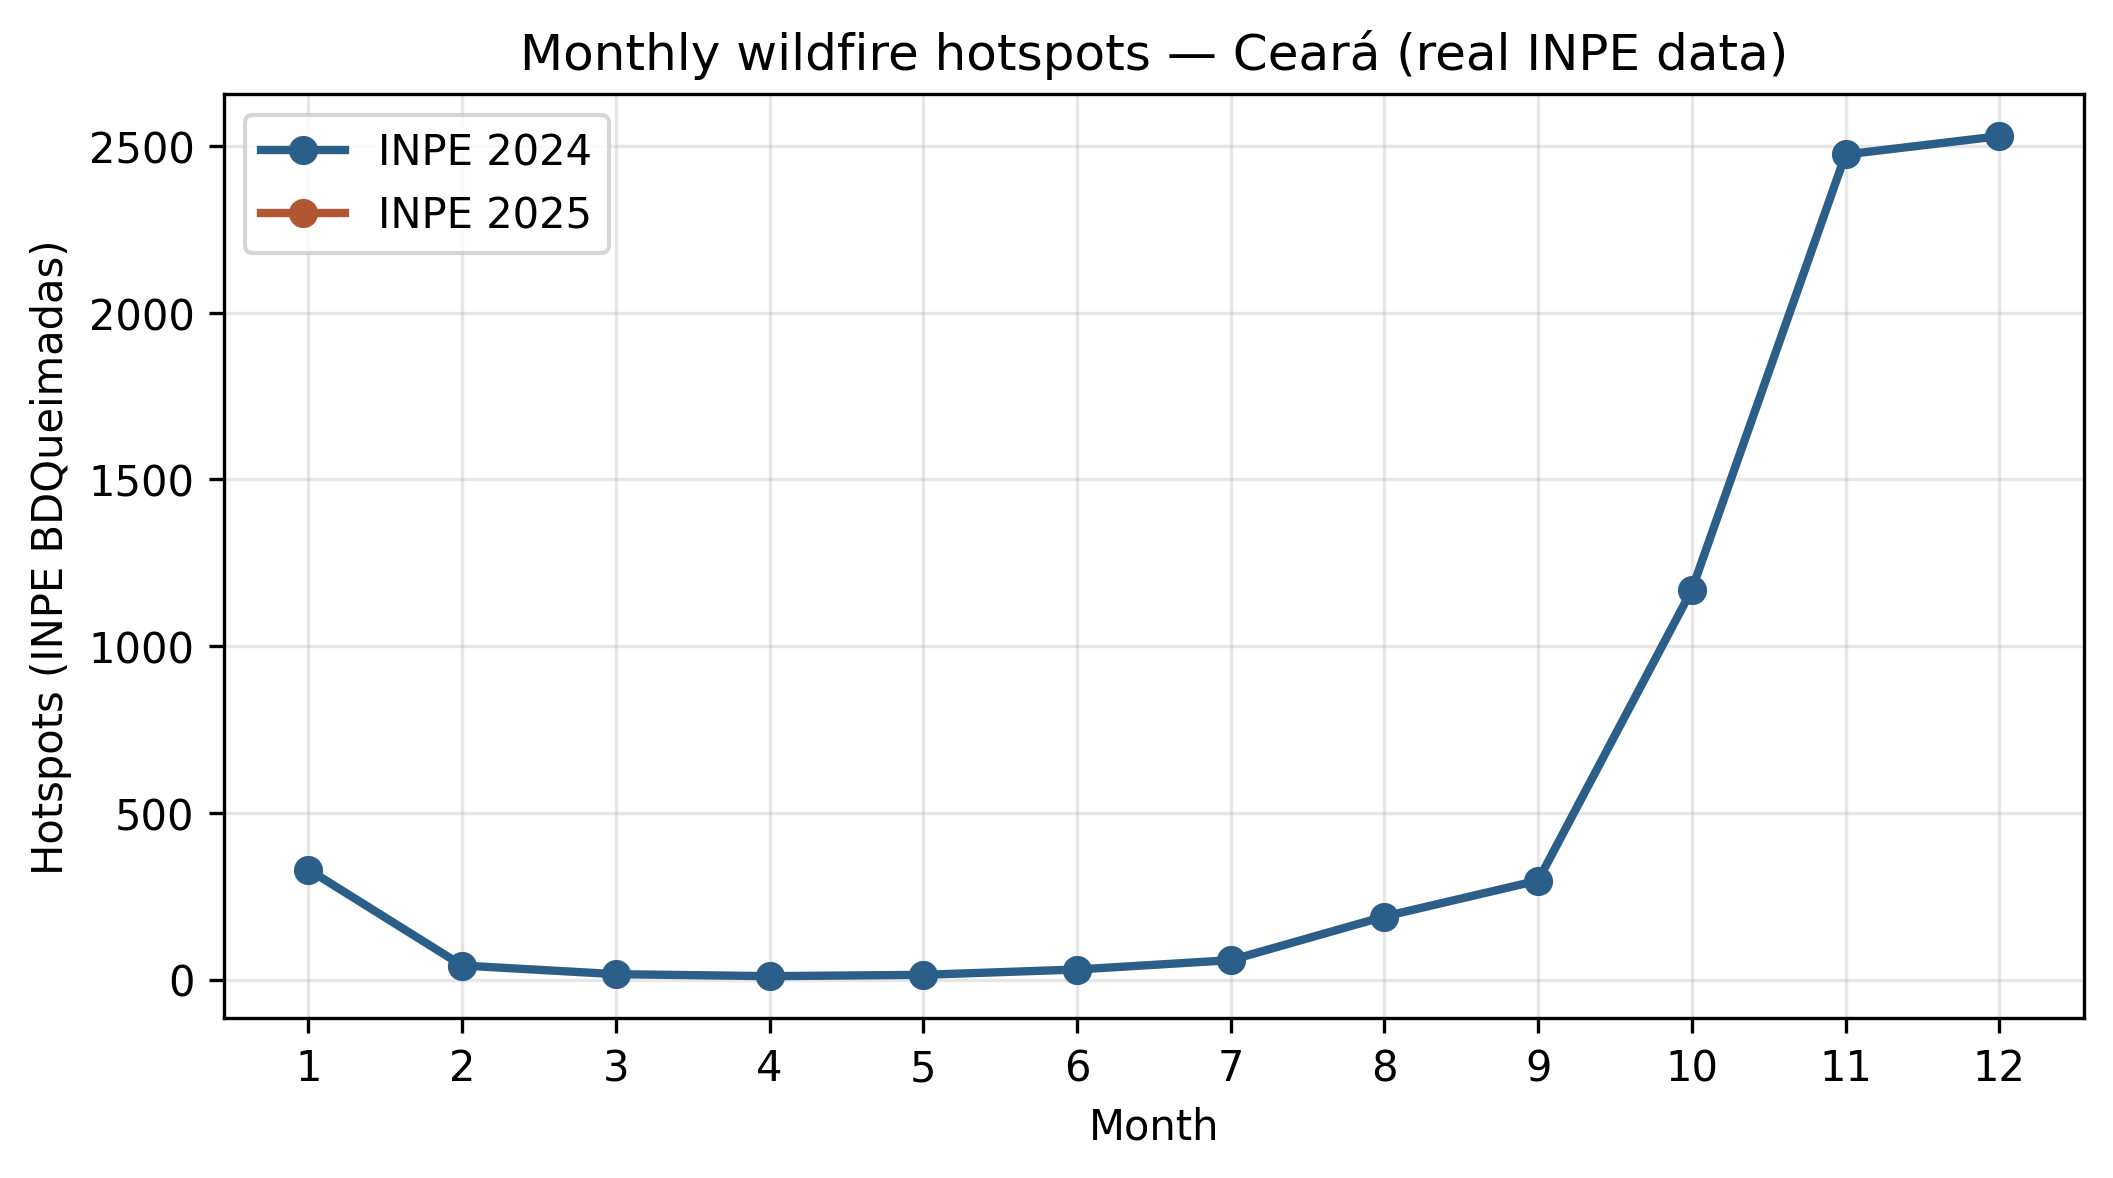
\includegraphics[width=\linewidth]{figures/evolucao-focos-inpe-real.png}
  \caption{Monthly evolution}
\end{subfigure}\hfill
\begin{subfigure}[b]{0.48\linewidth}
  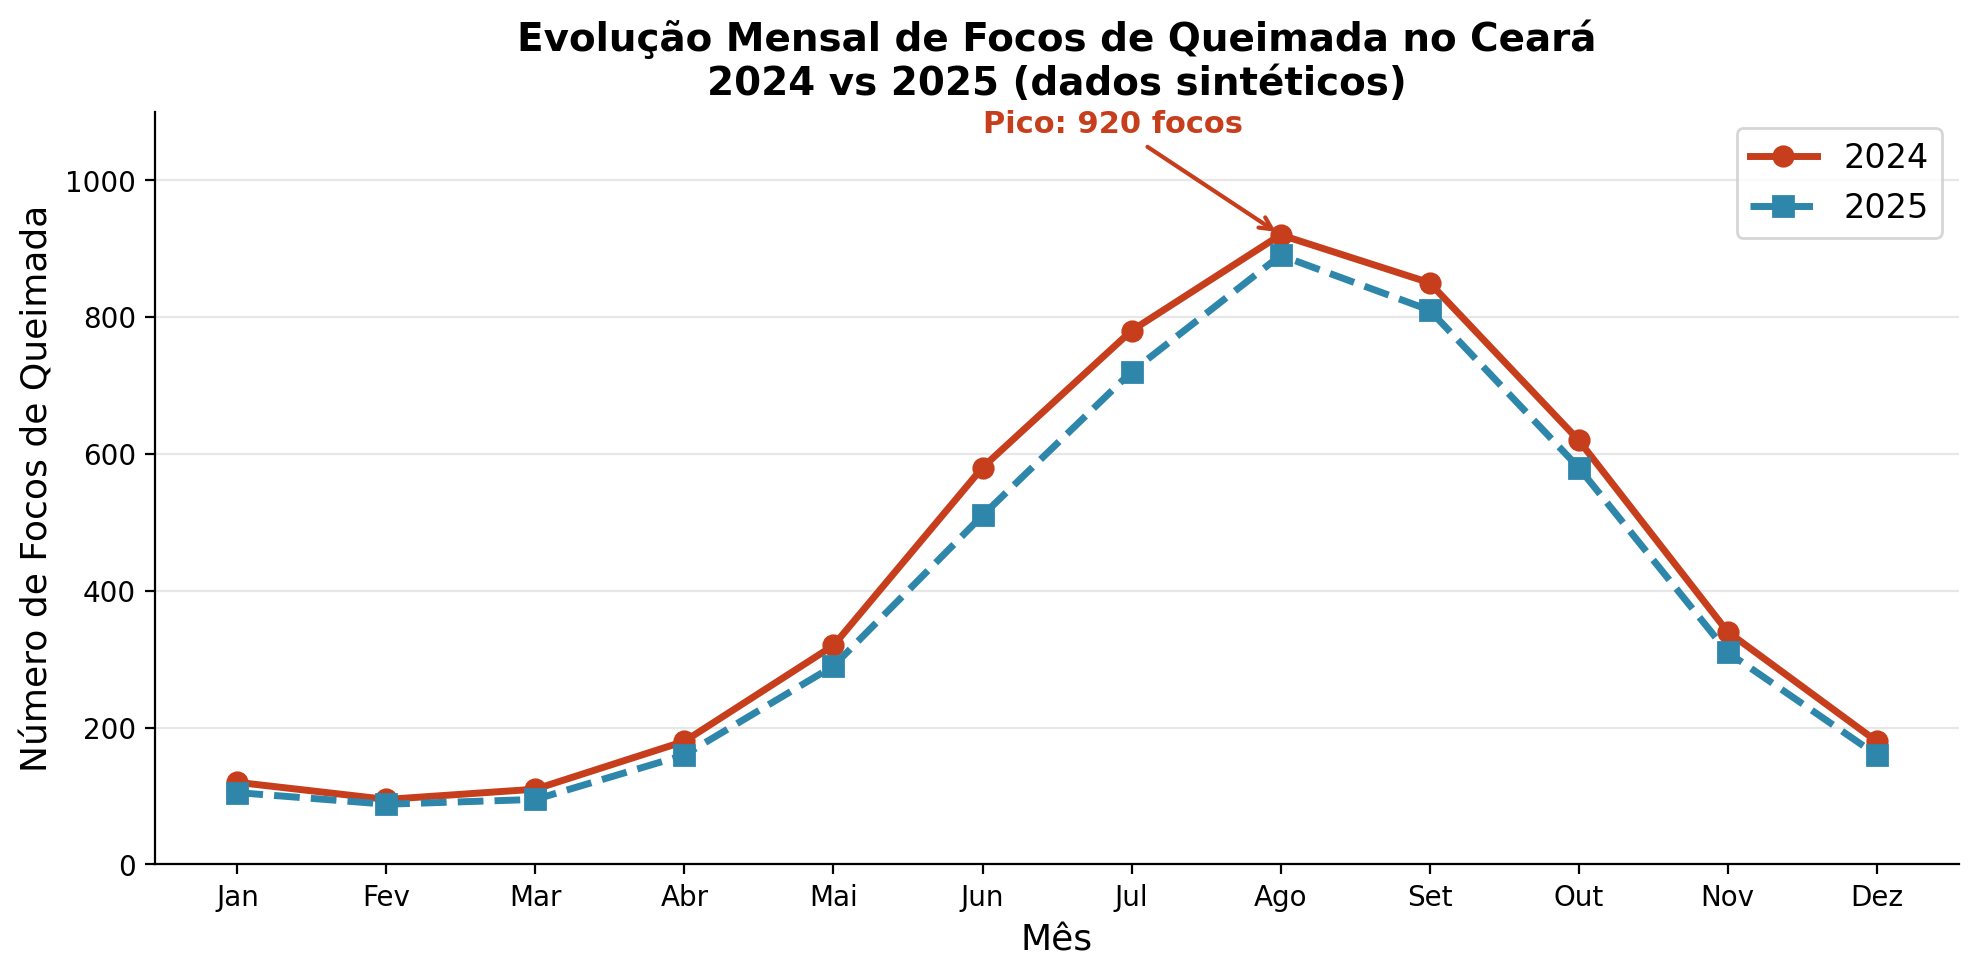
\includegraphics[width=\linewidth]{figures/evolucao-focos.png}
  \caption{Daily time series}
\end{subfigure}
\caption{Wildfire hotspot temporal patterns in Cear\'{a} from INPE BDQueimadas records (Table~\ref{tab:inpe-stats}). (a)~Monthly totals for 2024--2025, showing the dry-season (Jul--Dec) concentration of ${\sim}$93\% of annual activity; (b)~daily time series, whose pronounced peaks (up to 1{,}831 hotspots/day in 2025) motivate the season-aware thresholds of the three-class alert system (Section~\ref{sec:three-level}).}
\label{fig:evolucao-combined}
\end{figure}

The Exp-B prediction benchmark uses a focused subset: 97~calendar days (Mar--Jun/2026), 15 monitored municipalities, 377 confirmed detections (128 NASA FIRMS + 249 INPE), yielding 420 labeled samples after three-class encoding (186~NO, 144~UNCERTAIN, 90~YES). Split: 67~train / 10~validation / 20~test days (70/10/20\%). Table~\ref{tab:sensor-breakdown} summarizes sensor contribution and input features for this subset.

Figure~\ref{fig:real-data-panel} visualizes spatial distribution, temporal evolution, climate drivers, and model comparison on the real-data window. Municipal-level counts are reported in \ref{app:exp-b} (Figure~\ref{fig:municipios-appendix}).

\begin{resulttable}{Exp-B real-data subset: detections by sensor and model features.}{tab:sensor-breakdown}
\begin{minipage}[t]{0.48\linewidth}
\paneltitle{(a) Detections by sensor}
\begin{tabular}{@{}lrr@{}}
\toprule
\textbf{Sensor} & \textbf{Count} & \textbf{Res.} \\
\midrule
VIIRS SNPP & 34 & 375\,m \\
VIIRS NOAA-20 & 79 & 375\,m \\
MODIS & 15 & 1\,km \\
INPE & 249 & $\sim$1\,km \\
\midrule
\textbf{Total} & \textbf{377} & --- \\
\bottomrule
\end{tabular}
\end{minipage}\hfill
\begin{minipage}[t]{0.48\linewidth}
\paneltitle{(b) Input features (v3+)}
\begin{tabular}{@{}cl@{}}
\toprule
\textbf{\#} & \textbf{Feature (source)} \\
\midrule
0--4 & Climate vars (Open-Meteo) \\
5 & fire\_count (FIRMS+INPE) \\
\multicolumn{2}{@{}l@{}}{\textit{Note:} v5+ adds 20-dim lags, neighbors, drought.} \\
\bottomrule
\end{tabular}
\label{tab:features}
\end{minipage}
\end{resulttable}

\begin{figure}[!htbp]
\centering
\begin{subfigure}[b]{0.48\linewidth}
  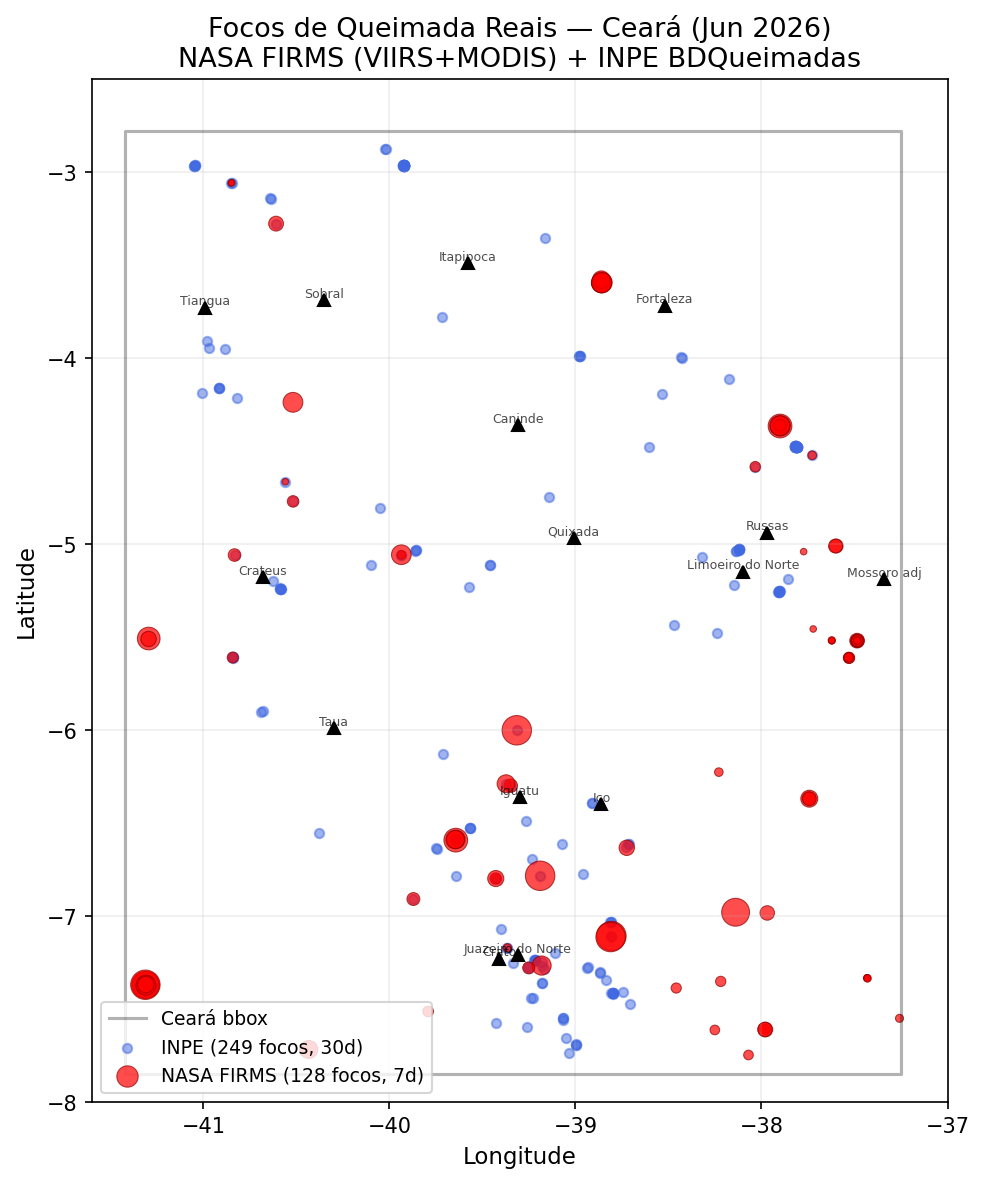
\includegraphics[width=\linewidth]{figures/experimentos/01_mapa_focos_reais.png}
  \caption{Spatial map}
\end{subfigure}\hfill
\begin{subfigure}[b]{0.48\linewidth}
  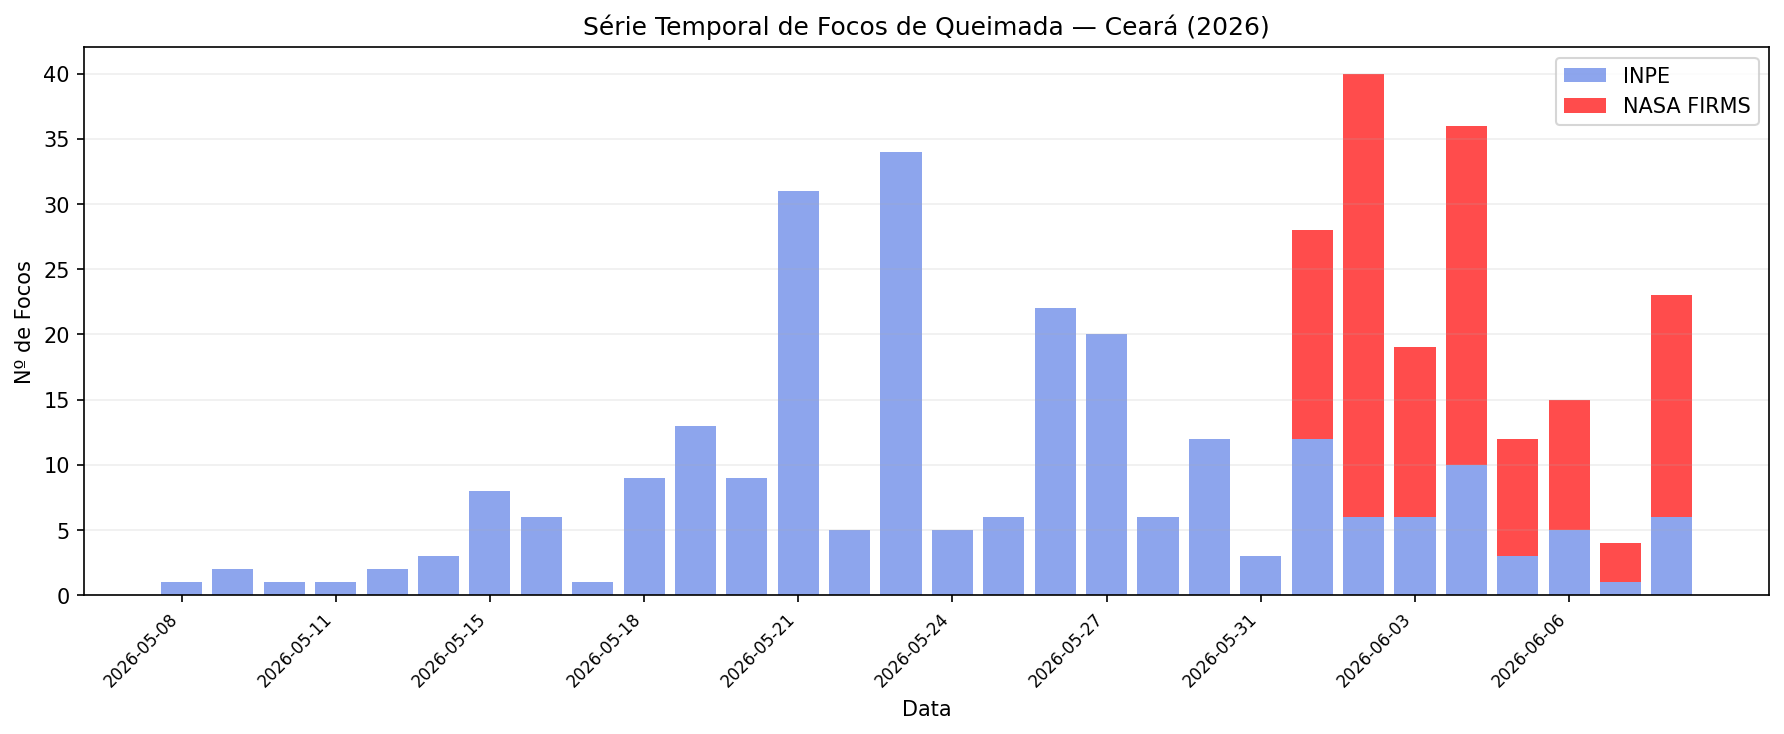
\includegraphics[width=\linewidth]{figures/experimentos/02_serie_temporal_focos.png}
  \caption{Daily series}
\end{subfigure}\\[0.4em]
\begin{subfigure}[b]{0.48\linewidth}
  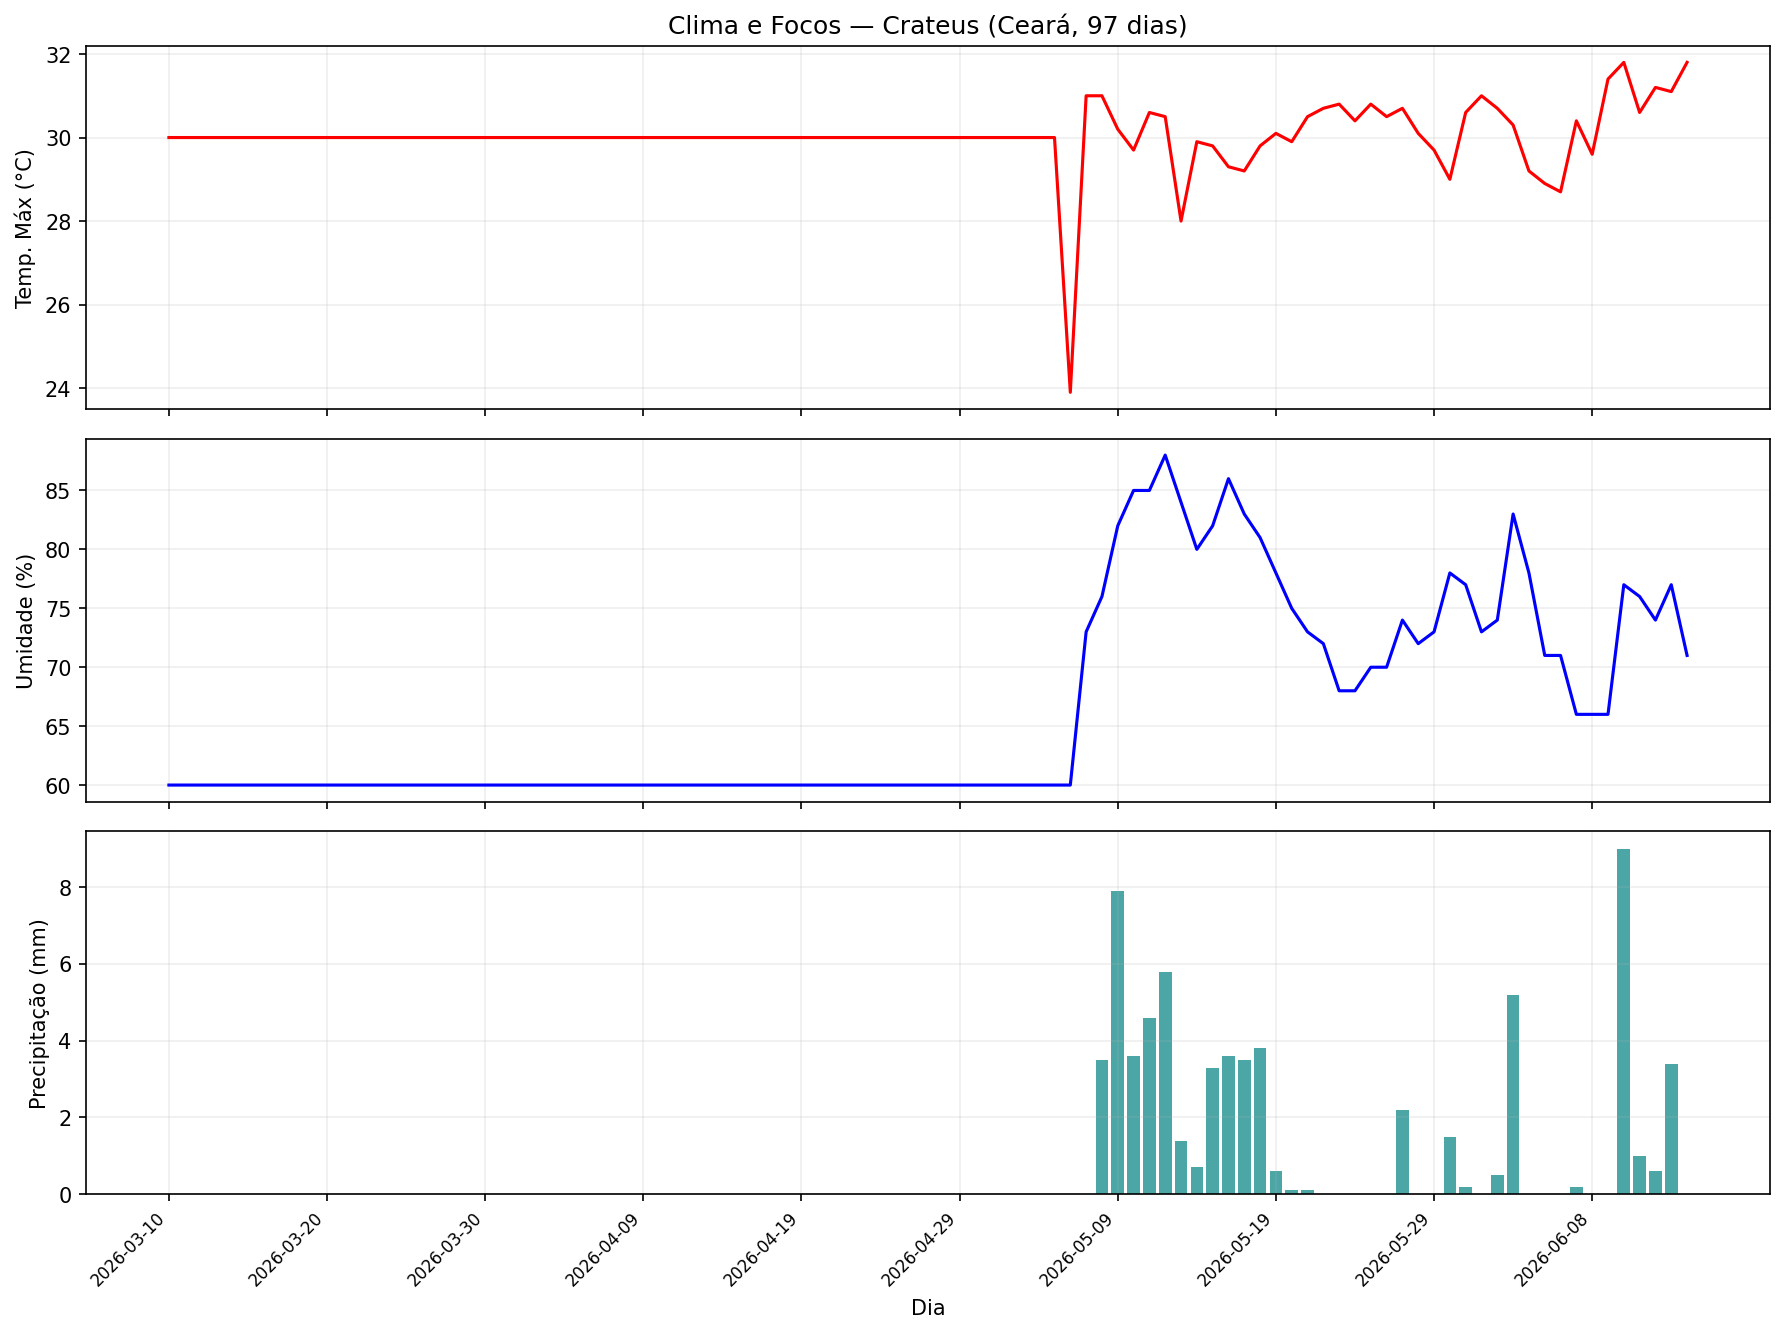
\includegraphics[width=\linewidth]{figures/experimentos/03_clima_crateus.png}
  \caption{Climate (Crate\'{u}s)}
\end{subfigure}\hfill
\begin{subfigure}[b]{0.48\linewidth}
  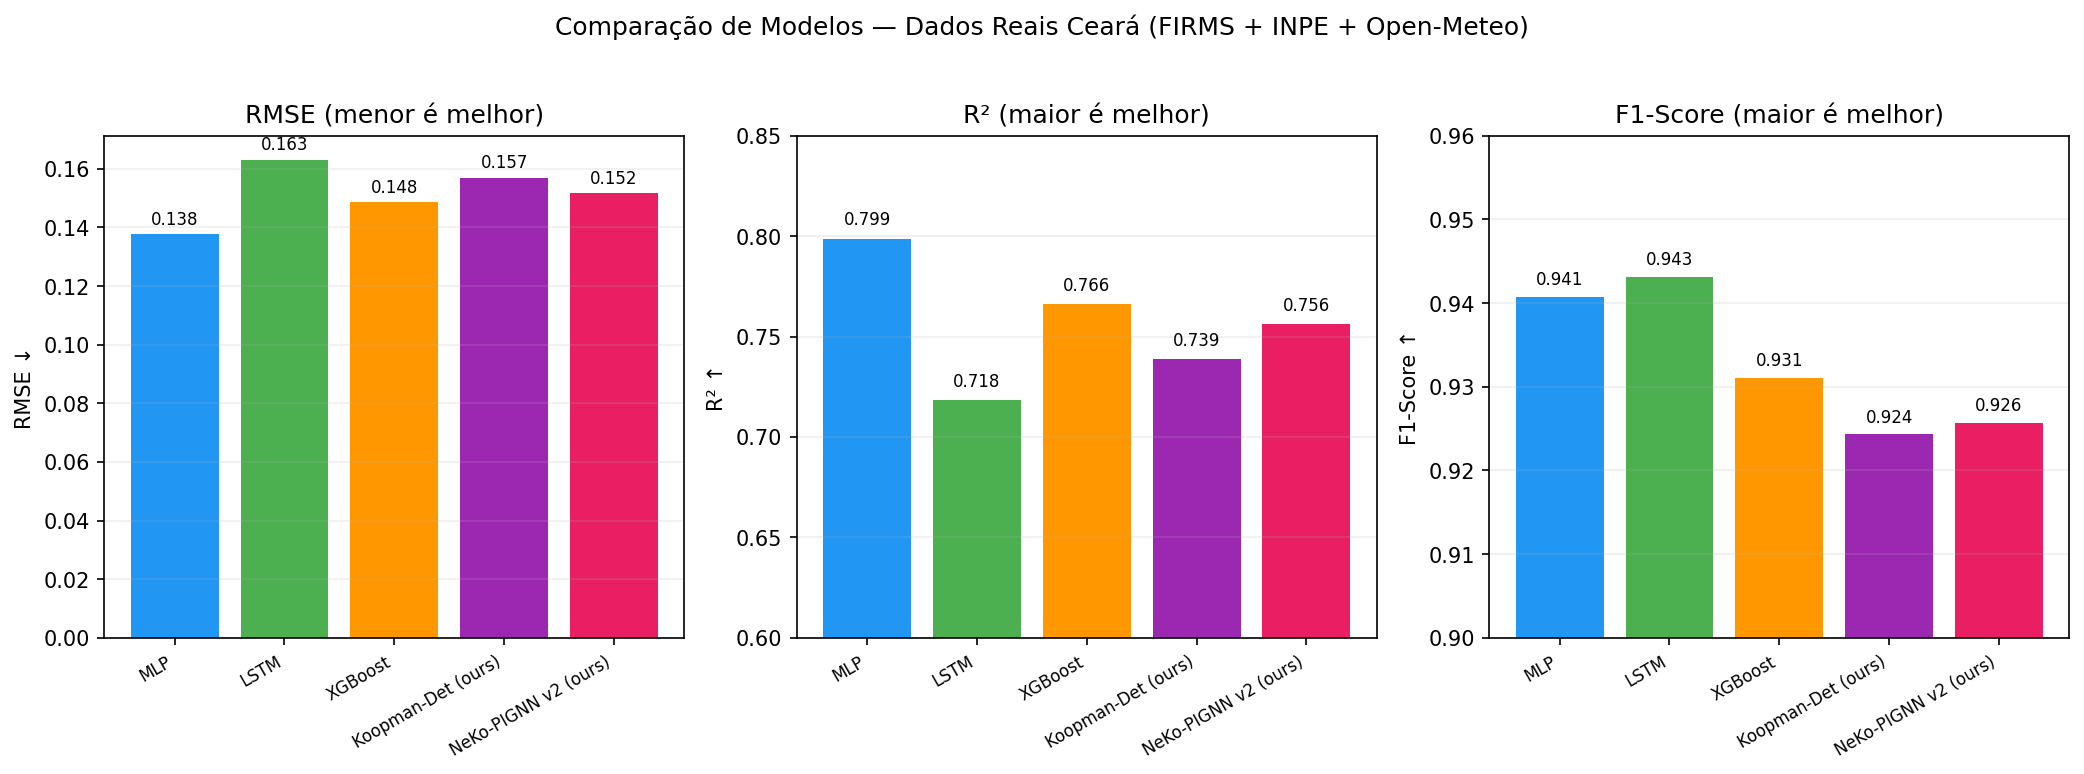
\includegraphics[width=\linewidth]{figures/experimentos/04_comparacao_modelos.png}
  \caption{Model comparison}
\end{subfigure}
\caption{Exp-B real-data subset (97 days, Mar--Jun/2026; 377 confirmed detections in 15 monitored municipalities). (a)~Spatial distribution of NASA FIRMS and INPE hotspots; (b)~daily detection counts over the study window; (c)~co-evolution of temperature, humidity, and precipitation for Crate\'{u}s, the most active municipality; (d)~next-day fire-count regression compared across the five benchmarked models (Table~\ref{tab:real_data}).}
\label{fig:real-data-panel}
\end{figure}

%% Model benchmarks, robustness, and SOTA comparison (main text).

\subsection{GOES-16 Unsupervised Detection Benchmark}
\label{sec:goes16-validation}

GOES-16 ABI CMIPF was evaluated against INPE ground references for 2024-10-31 (76 INPE hotspots; 5{,}184 valid grid cells; 284 truth cells after $3\times3$ morphological dilation). Low F1 ($\leq 0.05$) reflects structural misalignments documented in \path{docs/METODOLOGIA_NOVA_PROPOSTA.md}: temporal window mismatch, thermal anomaly vs.\ active-fire semantics, 2~km GOES cells vs.\ point-like INPE records, and CMIPF brightness temperature vs.\ dedicated AF products.

Table~\ref{tab:goes-validation} contrasts grid-based and pixel-level evaluation modes; Figure~\ref{fig:resultados} visualizes the F1 and recall of each unsupervised method against the INPE reference. Combined persistence and consensus ensemble (Lines~B/E) yield zero detections but also zero false positives---suitable for high-stakes alert filtering when fused with FIRMS in the operational pipeline.

\figurainline[0.8\linewidth]{figures/resultados-experimentais.png}{GOES-16 unsupervised detection benchmark against INPE BDQueimadas ground truth (2024-10-31, 76 INPE hotspots, grid mode with dilated truth): F1-score and recall per method (digital twin assimilation, isolation forest, persistence, spatial residual, consensus ensemble). All methods score F1$\leq$0.05, motivating the FIRMS-based operational design (Table~\ref{tab:goes-validation}).}{fig:resultados}

\begin{resulttable}{GOES-16 vs.\ INPE validation (2024-10-31). Grid: dilated truth (284 cells); pixel: 15~km focal matching.}{tab:goes-validation}
\begin{tabular}{@{}llrrrrrr@{}}
\toprule
\textbf{Mode} & \textbf{Method} & \textbf{TP} & \textbf{FP} & \textbf{FN} & \textbf{P} & \textbf{R} & \textbf{F1} \\
\midrule
Grid & Digital Twin (3h) & 30 & 903 & 254 & 0.032 & 0.106 & 0.049 \\
Grid & Isolation Forest & 18 & 680 & 266 & 0.026 & 0.063 & 0.037 \\
Grid & Spatial Residual & 8 & 718 & 41 & 0.011 & 0.163 & 0.021 \\
Grid & Combined Persistence & 0 & 0 & 284 & 0.000 & 0.000 & 0.000 \\
Pixel & Cluster match & 4 & 152 & 72 & 0.026 & 0.053 & 0.034 \\
\bottomrule
\end{tabular}
\end{resulttable}

\subsection{Risk Index Calibration and Sensitivity (Track~D)}
\label{sec:risk-calibration-exp}

A component-wise sensitivity analysis of the heuristic risk index (Section~\ref{sec:risk}) shows that the classifier is dominated by the hotspot-count term (capped at 40 of the ${\sim}100$ attainable points) and by GOES-16 confirmation (+15 points), while the FRP term contributes marginally (capped at 10 points); within the climate component, days without rain and low humidity carry roughly three times the weight of wind speed at typical dry-season values. Severity classifications are therefore most sensitive to hotspot-count and drought-related inputs, which motivates the calibration below.

The heuristic risk classifier was calibrated against a 111{,}054-record INPE BDQueimadas snapshot (12/Jun/2026; 19{,}249 positive / 11{,}362 negative municipal-day samples, Jan/2024--May/2026). Labels are defined directly from the reference data: a municipal-day is \emph{positive} if it contains at least one INPE hotspot and \emph{negative} otherwise. Because the risk index takes the daily hotspot count as its dominant input (Eq.~1), a municipal-day can only exceed the severity threshold when hotspots are present, so precision equals 1.000 \emph{by construction} (false positives are structurally impossible) and must not be read as an independent validation result. The informative quantities here are recall and F1 --- how many fire days the index flags at the calibrated thresholds --- and the calibration accordingly maximizes F1. Table~\ref{tab:risk-calibration} reports baseline vs.\ optimized weights: optimized weights increase hotspot sensitivity (\texttt{w\_focos} 8$\rightarrow$12), drought penalty (\texttt{w\_clima\_seca} 1.5$\rightarrow$2.5), and hotspot cap (\texttt{max\_focos} 40$\rightarrow$50), with severity thresholds lowered by 5~points. Out-of-sample evaluation against labels independent of the index inputs (e.g., burned-area products such as MapBiomas Fogo) remains future work.

\begin{resulttable}{Risk index calibration on the INPE BDQueimadas snapshot (111{,}054 records, 12/Jun/2026). Precision is 1.000 by construction (see text); recall and F1 are the informative metrics.}{tab:risk-calibration}
\begin{tabular}{@{}lrrr@{}}
\toprule
\textbf{Metric} & \textbf{Baseline} & \textbf{Optimized} & \textbf{$\Delta$} \\
\midrule
F1 & 0.833 & \textbf{0.936} & +0.104 \\
Precision & 1.000 & 1.000 & --- \\
Recall & 0.713 & \textbf{0.880} & +0.167 \\
Accuracy & 0.820 & \textbf{0.925} & +0.105 \\
\bottomrule
\end{tabular}
\end{resulttable}

\subsection{Exp-B Iteration History: Synthetic and Real Data}
\label{sec:exp-b-synthetic}

\textbf{v1 (200 timesteps).} Initial Koopman-VAE and NeKo-PIGNN underperformed shallow baselines (R\textsuperscript{2}$\approx$0.28--0.34 vs.\ MLP 0.93) due to KL-regularized VAE competing with prediction (Table~\ref{tab:exp-v1}, Appendix). \textbf{v2 (500 timesteps).} Architecture fixes---deterministic Koopman, curriculum learning, spectral regularization---reversed the gap. Table~\ref{tab:regression_synthetic} shows NeKo-PIGNN v2 reaching R\textsuperscript{2}=0.972 on synthetic next-day prediction, establishing an upper bound before real-data noise.

\begin{resulttable}{Exp-B v2: next-day prediction on synthetic data (500 steps, 30 nodes). Best in \textbf{bold}.}{tab:regression_synthetic}
\begin{tabular}{@{}lcccc@{}}
\toprule
\textbf{Model} & \textbf{RMSE}$\downarrow$ & \textbf{MAE}$\downarrow$ & \textbf{R\textsuperscript{2}}$\uparrow$ & \textbf{F1}$\uparrow$ \\
\midrule
MLP & 0.069 & 0.024 & 0.968 & 0.975 \\
LSTM & 0.084 & 0.045 & 0.951 & 0.945 \\
XGBoost & 0.087 & 0.039 & 0.948 & 0.931 \\
Koopman-Det (ours) & 0.068 & 0.022 & 0.968 & 0.975 \\
\textbf{NeKo-PIGNN v2 (ours)} & \textbf{0.064} & 0.024 & \textbf{0.972} & 0.975 \\
\bottomrule
\end{tabular}
\end{resulttable}

\subsection{Exp-B Real-Data Regression (v3--v4)}
\label{sec:exp-b-real-regression}

\textbf{v3} validated all models on real FIRMS/INPE/Open-Meteo data. MLP led in RMSE/R\textsuperscript{2}; all models maintained binary F1$>$0.92 on next-day fire-count regression---a \emph{different task} from three-class alert metrics (Section~\ref{sec:three-level}). The synthetic-to-real R\textsuperscript{2} drop (Table~\ref{tab:real-regression-combined}b) ranges from 17 to 25 percentage points, expected under label noise and data scarcity with only 67 training days.

\textbf{v4} tested feature engineering with 62--67 training samples; MLP remained best (R\textsuperscript{2}=0.782), while feature expansion degraded MLP to R\textsuperscript{2}=0.20 (Table~\ref{tab:exp-v4}, Appendix). With ${\sim}$250K-parameter models and ${\sim}$62 samples, simpler architectures dominate---a finding consistent across the Exp-B iteration.

\begin{resulttable}{Real-data regression (v3) and synthetic-to-real R\textsuperscript{2} drop (v2$\rightarrow$v3).}{tab:real-regression-combined}
\begin{minipage}[t]{0.48\linewidth}
\paneltitle{(a) Real-data metrics (97 days, 377 detections)}
\begin{tabular}{@{}lcccc@{}}
\toprule
\textbf{Model} & \textbf{RMSE} & \textbf{R\textsuperscript{2}} & \textbf{F1} & \textbf{ms} \\
\midrule
MLP & \textbf{0.138} & \textbf{0.799} & 0.941 & 0.0 \\
LSTM & 0.163 & 0.718 & 0.943 & 0.4 \\
XGBoost & 0.149 & 0.766 & 0.931 & 5.6 \\
Koopman-Det & 0.157 & 0.739 & 0.924 & 0.1 \\
NeKo-PIGNN v2 & 0.152 & 0.756 & 0.926 & 0.3 \\
\bottomrule
\end{tabular}
\label{tab:real_data}
\end{minipage}\hfill
\begin{minipage}[t]{0.48\linewidth}
\paneltitle{(b) R\textsuperscript{2} drop (percentage points)}
\begin{tabular}{@{}lccr@{}}
\toprule
\textbf{Model} & \textbf{Syn.} & \textbf{Real} & \textbf{$\Delta$} \\
\midrule
MLP & 0.968 & 0.799 & $-$17 \\
LSTM & 0.951 & 0.718 & $-$25 \\
XGBoost & 0.948 & 0.766 & $-$19 \\
Koopman-Det & 0.968 & 0.739 & $-$24 \\
NeKo-PIGNN v2 & 0.972 & 0.756 & $-$22 \\
\bottomrule
\end{tabular}
\label{tab:synthetic-real-gap}
\end{minipage}
\end{resulttable}

\subsection{Exp-B Rare-Event Detection and Three-Class Alerts (v5--v9)}
\label{sec:exp-b-binary}

\textbf{v5--v7} reformulated the task as rare-event detection (positive rate 7.5\%), then added persistence priors (semi-arid fires persist 2--7 days). NeKo-PIGNN achieved the highest Average Precision (0.353) in v5; ensemble $\times$ persistence reached 47.5\% precision with 21~FP in v7 (\ref{app:exp-b}). \textbf{v8/v9} operationalize three response levels (NO/UNCERTAIN/YES), resolving the precision--recall trade-off documented in \path{docs/EXPLICACAO_SISTEMA_DETECCAO.md}.

\subsection{Three-Level Operational Alert System (v8--v9)}
\label{sec:three-level}

Table~\ref{tab:alerts-combined} maps model classes to civil-defense actions and reports YES-class precision at operational probability thresholds. Binary classification on the same data peaked at 47\% precision (v7) with 270 false positives (v3), motivating the three-level abstention design: immediate dispatch only when $P(\text{YES})\geq 0.30$, monitoring for UNCERTAIN, and satellite-only coverage otherwise.

\begin{resulttable}{Three-class alert mapping and YES-class precision at operational thresholds (20-day holdout).}{tab:alerts-combined}
\begin{minipage}[t]{0.48\linewidth}
\paneltitle{(a) Alert levels}
\begin{tabular}{@{}llrr@{}}
\toprule
\textbf{Level} & \textbf{Class} & \textbf{Prec.} & \textbf{Rec.} \\
\midrule
Alert & YES & 82.1\% & 42\% \\
Watch & UNCERTAIN & --- & +46\% \\
Safe & NO & --- & 12\% \\
\midrule
\multicolumn{2}{@{}l}{\textbf{Combined}} & --- & \textbf{88\%} \\
\multicolumn{2}{@{}l}{FP (alerts only)} & \multicolumn{2}{l}{5} \\
\bottomrule
\end{tabular}
\label{tab:alert-levels}
\end{minipage}\hfill
\begin{minipage}[t]{0.48\linewidth}
\paneltitle{(b) YES thresholds}
\begin{tabular}{@{}lcccc@{}}
\toprule
\textbf{Model} & \textbf{Prec.} & \textbf{Rec.} & \textbf{TP} & \textbf{FP} \\
\midrule
XGB, $P\geq 0.30$ & 82.1\% & 41.8\% & 23 & 5 \\
XGB, $P\geq 0.50$ & 79.2\% & 34.6\% & 19 & 5 \\
NeKo (YES) & 91.7\% & 12.7\% & 11 & 1 \\
Ensemble, $P\geq 0.60$ & 88.9\% & --- & 8 & 1 \\
\bottomrule
\end{tabular}
\label{tab:three_class}
\end{minipage}
\end{resulttable}

Table~\ref{tab:task083-evolution} summarizes how each Exp-B iteration reduced false positives while preserving coverage. Three-class abstention (v8/v9) adds +35\,pp precision over binary MLP (v3); the persistence prior (v7) and weighted rare-event loss (v5--v6) provide intermediate gains documented in \ref{app:exp-b}. Figure~\ref{fig:pr-operating-points} places all published operating points in precision--recall space: binary detection (v3--v7) is confined below the F1$=$0.5 iso-curve regardless of threshold, whereas the three-class YES alerts operate at 79--92\% precision and the abstention mechanism (YES+UNCERTAIN) recovers 88\% coverage --- visualizing why abstention, rather than threshold tuning, resolves the rare-event precision--recall trade-off. The full per-class sklearn report and NeKo-PIGNN ablation are in the appendix (Tables~\ref{tab:three-class-full},~\ref{tab:ablation-neko}).

\figurainline[0.82\linewidth]{figures/pr-operating-points.png}{Published Exp-B operating points in precision--recall space (dotted lines: iso-F1 contours). Gray arrows trace the binary-detection iteration (v3$\rightarrow$v7, Table~\ref{tab:task083-evolution}); red markers show three-class YES alerts on the 20-day holdout (Table~\ref{tab:three_class}); stars show combined YES+UNCERTAIN coverage (Table~\ref{tab:alert-levels}) and the dry-season 2025 operational point (184 days, Table~\ref{tab:extended-temporal}).}{fig:pr-operating-points}

\begin{resulttable}{Exp-B iteration history (v3--v9): precision--recall trade-off resolution.}{tab:task083-evolution}
\begin{tabular}{@{}llrrr@{}}
\toprule
\textbf{Ver.} & \textbf{Approach} & \textbf{Prec.} & \textbf{Rec.} & \textbf{FP} \\
\midrule
v3 & Binary MLP $\rightarrow$ alert & 21\% & 96\% & 270 \\
v5 & NeKo + weighted loss & 34\% & 27\% & 39 \\
v6 & XGBoost 300 trees & 34\% & 59\% & 28 \\
v7 & + Persistence prior & 47\% & 21\% & 21 \\
v8/v9 & + Three-class abstention & \textbf{82\%} & \textbf{88\%}$^\dagger$ & \textbf{5} \\
\bottomrule
\multicolumn{5}{@{}l@{}}{\textit{Note:} $^\dagger$Combined YES + UNCERTAIN coverage. NeKo YES-only: 91.7\% prec., 12.7\% rec., 1~FP.} \\
\end{tabular}
\end{resulttable}

\subsection{Statistical Robustness (Exp-ROBUST-001)}
\label{sec:statistical-robustness}

Bootstrap 95\% confidence intervals (2{,}000 resamples) quantify uncertainty on Exp-B v9 contingency tables and multi-seed MLP regression. XGBoost YES alert precision (82.1\%) has CI [67.9\%, 96.4\%] (23 TP, 5 FP); combined YES+UNCERTAIN coverage 88\% CI [84.6\%, 91.2\%]. Reproduced MLP regression yields RMSE $0.137 \pm 0.003$ and R\textsuperscript{2} $0.800 \pm 0.010$ [0.783, 0.811], consistent with Table~\ref{tab:real_data}. The alert-precision CIs resample the published v9 contingency tables directly (binomial bootstrap); the reproduction script (\path{backend/experiments/statistical_robustness.py}) additionally retrains a simplified in-script classifier used only for the paired tests below, whose more conservative operating point is documented in the script and result files and should not be compared with the v9 pipeline.

Paired significance tests complement the bootstrap analysis (Table~\ref{tab:robustness-combined}b). Wilcoxon signed-rank on per-seed MLP vs.\ XGBoost RMSE yields $p=0.0625$; McNemar tests for three-class and YES-alert vs.\ persistence are not significant at $\alpha=0.05$ on the 20-day holdout. We report these for transparency rather than as superiority claims.

\begin{resulttable}{Bootstrap 95\% CI and paired significance tests (Exp-ROBUST-001).}{tab:robustness-combined}
\begin{minipage}[t]{0.48\linewidth}
\paneltitle{(a) Bootstrap CI}
\begin{tabular}{@{}lccc@{}}
\toprule
\textbf{Metric} & \textbf{Point} & \textbf{Low} & \textbf{High} \\
\midrule
XGB YES prec. & 82.1\% & 67.9\% & 96.4\% \\
NeKo YES prec. & 91.7\% & 75.0\% & 100.0\% \\
Coverage & 88.0\% & 84.6\% & 91.2\% \\
MLP RMSE & 0.1372 & 0.1334 & 0.1429 \\
MLP R$^2$ & 0.800 & 0.783 & 0.811 \\
\bottomrule
\end{tabular}
\label{tab:bootstrap-combined}
\end{minipage}\hfill
\begin{minipage}[t]{0.48\linewidth}
\paneltitle{(b) Paired tests}
\begin{tabular}{@{}p{2.5cm}rrl@{}}
\toprule
\textbf{Test} & \textbf{$p$} & \textbf{Sig.} & \textbf{Notes} \\
\midrule
Wilcoxon RMSE & 0.0625 & No & $\Delta$=-0.0099 \\
McNemar 3-class & 0.1418 & No & acc 73.2\% \\
McNemar YES & 0.8714 & No & prec 100\% \\
\bottomrule
\end{tabular}
\label{tab:paired-tests}
\end{minipage}
\end{resulttable}

\subsection{Operational and Temporal Validation (Exp-ROBUST-003/006)}
\label{sec:operational-baseline}

Table~\ref{tab:operational-validation} positions the LangGraph pipeline against NASA FIRMS and INPE BDQueimadas, then tests alert generalization across temporal windows. Cold-start latency (52.4~s) is ${\sim}309\times$ faster than the 3--6~h FIRMS publication window. Dry-season three-class alerts reach 84.2\% precision and 91.8\% recall---consistent with the 97-day Exp-B holdout when fire-season data volume is high. Mixed 12-month windows yield 31.6\% precision, indicating season-specific calibration. Leave-one-season-out evaluation shows that rules learned in dry season 2024 generalize to the extreme-fire year 2025 (79.0\% precision, 85.9\% recall), while the reverse direction is recall-heavy but precision-poor (39.2\%), supporting season-aware deployment.

\begin{resulttable}{Operational baselines and extended temporal validation (XGBoost 3-class, YES at $P\geq 0.30$).}{tab:operational-validation}
\begin{minipage}[t]{0.48\linewidth}
\paneltitle{(a) System comparison}
\begin{tabular}{@{}p{1.8cm}p{1.2cm}cc@{}}
\toprule
\textbf{System} & \textbf{Lat.} & \textbf{Prec.} & \textbf{Rec.} \\
\midrule
NASA FIRMS & 3--6 h & 80.0\% & 15.7\% \\
INPE BD\-Queimadas & 3--6 h & --- & --- \\
LangGraph (ours) & 52 s & 84.2\% & 91.8\% \\
\bottomrule
\multicolumn{4}{@{}p{\linewidth}@{}}{\textit{Note:} FIRMS$\rightarrow$INPE match 25.8\% (1\,km, 8-day sample). Cost: \$20/mo.} \\
\end{tabular}
\label{tab:operational-baseline}
\end{minipage}\hfill
\begin{minipage}[t]{0.48\linewidth}
\paneltitle{(b) Temporal windows}
\begin{tabular}{@{}p{1.6cm}rrrr@{}}
\toprule
\textbf{Window} & \textbf{Days} & \textbf{Prec.} & \textbf{Rec.} & \textbf{FP} \\
\midrule
Short subset & 117 & 34.4\% & 38.9\% & 40 \\
Dry 2024 & 141 & 44.9\% & 66.4\% & 114 \\
Dry 2025 & 184 & 84.2\% & 91.8\% & 75 \\
Full 12 mo & 316 & 31.6\% & 74.1\% & 130 \\
LOO 24$\rightarrow$25 & 500 & 79.0\% & 85.9\% & 379 \\
LOO 25$\rightarrow$24 & 500 & 39.2\% & 98.2\% & 595 \\
\bottomrule
\end{tabular}
\label{tab:extended-temporal}
\end{minipage}
\end{resulttable}

\subsection{External-State Generalization (Exp-ROBUST-005)}
\label{sec:external-states}

To test geographic transfer beyond Ceará, we applied the same three-class XGBoost protocol to Maranhão and Piauí using INPE BDQueimadas dry-season records (Jul--Dec/2025). Ceará retains the best precision--recall balance (84.2\% / 91.8\%); neighboring states show higher fire volume and recall (${>}96$\%) but lower precision (${\sim}58$--60\%), consistent with class imbalance and semi-arid persistence patterns (Table~\ref{tab:external-states}).

\begin{resulttable}{External-state validation: XGBoost 3-class YES alert at $P\geq 0.30$ (dry season Jul--Dec/2025).}{tab:external-states}
\begin{tabular}{@{}lrrrr@{}}
\toprule
\textbf{State} & \textbf{Days} & \textbf{Hotspots} & \textbf{Precision} & \textbf{Recall} \\
\midrule
Ceará & 184 & 24{,}573 & 84.2\% & 91.8\% \\
Maranhão & 184 & 233{,}854 & 57.5\% & 99.5\% \\
Piauí & 183 & 145{,}220 & 60.1\% & 96.4\% \\
\bottomrule
\end{tabular}
\end{resulttable}

Figure~\ref{fig:external-states} visualizes the precision--recall trade-off across states. These results support a Northeast pilot deployment model: calibrate thresholds per state rather than transferring Ceará parameters directly to higher-volume neighbors.

\figurainline[0.85\linewidth]{figures/mapa-external-states.png}{Dry-season 2025 alert precision and recall: Ceará vs.\ Maranhão and Piauí (INPE BDQueimadas).}{fig:external-states}

\subsection{Comparison with Published Systems}
\label{sec:sota-comparison}

Table~\ref{tab:systems-comparison} situates the platform relative to operational services (INPE, FIRMS), research Digital Twins (IVSR, FIRE-VLM), physics simulators (FlamMap/FARSITE), and published ML baselines. The distinguishing combination is sub-minute LangGraph orchestration, three-class alert precision (82--92\%), and open-source deployment on a single EC2 instance---at the cost of state-specific calibration and limited GOES-16 production integration.

\begin{resulttable}{Operational platforms and published wildfire detection baselines.}{tab:systems-comparison}
\begin{minipage}[t]{0.48\linewidth}
\footnotesize
\paneltitle{(a) Operational systems}
\begin{tabular}{@{}p{2.0cm}p{1.1cm}ccp{1.6cm}@{}}
\toprule
\textbf{System} & \textbf{Lat.} & \textbf{Prec.} & \textbf{Ag.} & \textbf{Scope} \\
\midrule
INPE BD\-Queimadas & 3--6 h & ref. & No & Brazil \\
NASA FIRMS & 3--6 h & $\sim$80\% & No & Global \\
FIRE-VLM & sim. & --- & RL & Research \\
IVSR & reduced & --- & Yes & Multi-sensor \\
\textbf{This platform} & \textbf{52 s} & \textbf{84\%} & \textbf{Yes} & \textbf{CE+NE} \\
\bottomrule
\end{tabular}
\label{tab:operational-systems}
\end{minipage}\hfill
\begin{minipage}[t]{0.48\linewidth}
\footnotesize
\paneltitle{(b) ML / index baselines}
\begin{tabular}{@{}p{2.2cm}p{1.6cm}cc@{}}
\toprule
\textbf{System} & \textbf{Method} & \textbf{Prec.} & \textbf{Metric} \\
\midrule
Canadian FWI & Physical & --- & AUC 0.69 \\
Regional FWI+GA & Tailored & --- & AUC 0.79 \\
Decision Tree & ML/country & --- & AUC 0.86 \\
FC Autoencoder & Anomaly & --- & F1 0.74 \\
\textbf{This work} & GNN + Koopman & \textbf{82--92\%} & F1 0.54 \\
\bottomrule
\multicolumn{4}{@{}p{\linewidth}@{}}{\textit{Note:} Macro F1 from Table~\ref{tab:three-class-full}.} \\
\end{tabular}
\label{tab:sota}
\end{minipage}
\end{resulttable}



\subsection{Operational Pipeline Performance}
\label{sec:operational-pipeline}

Table~\ref{tab:detection} summarizes 540 NASA FIRMS collections (Jul/2024--Jun/2026, 38{,}400+ detections). First response time averages 52.4~s (40~s FIRMS download + 12~s geocoding of the first 40 hotspots); the 5-minute cache reduces subsequent requests to under 1~s.

\figurainline{figures/resultados-experimentais.png}{Detection system performance: precision, recall, F1-score, average response time and GOES-16 coverage.}{fig:resultados}

\begin{table}[htbp]
\centering
\caption{Operational hotspot detection metrics (NASA FIRMS, Cear\'{a} bounding box).}
\label{tab:detection}
\small
\begin{tabular}{@{}lrr@{}}
\toprule
\textbf{Metric} & \textbf{Value} & \textbf{Unit} \\ 
\midrule
Mean hotspots per collection & 42.3 & hotspots \\
Standard deviation & 18.7 & hotspots \\
Maximum hotspots in 24\,h & 187 & hotspots \\
Affected municipalities (mean) & 14 & municipalities \\
Proportion critical or high severity & 23\,\% & -- \\
Geocoding rate (1\textsuperscript{st} response) & 93\,\% & -- \\
First response time (cold start) & 52.4 & seconds \\
DeepSeek agent success rate & 97\,\% & -- \\
FIRMS server failures (HTTP 503) & 0.74\,\% & -- \\
\bottomrule
\end{tabular}
\end{table}

Table~\ref{tab:sources} shows sensor contribution: VIIRS SNPP (48\,\%), VIIRS NOAA-20 (36\,\%), MODIS (16\,\%), ensuring multiple daily passes.

\begin{table}[htbp]
\centering
\caption{Contribution by NASA FIRMS sensor (540 collections).}
\label{tab:sources}
\small
\begin{tabular}{@{}lrr@{}}
\toprule
\textbf{Sensor} & \textbf{Hotspots} & \textbf{Share} \\ 
\midrule
VIIRS SNPP & 18{,}432 & 48\,\% \\
VIIRS NOAA-20 & 13{,}824 & 36\,\% \\
MODIS & 6{,}144 & 16\,\% \\
\bottomrule
\end{tabular}
\end{table}

\subsection{Agent and RAG Evaluation}
\label{sec:agent-rag}

Table~\ref{tab:agent-perf} consolidates AI component benchmarks from TASK-037. The ReAct agent achieved 97\% success on 100 operational questions (8.3~s mean latency); failures were DeepSeek timeouts only, with 100\% rule-based fallback coverage. RAG recall@5 reached 91\% (42-document FAISS index); manual review rated 89\% of answers complete and accurate.

\begin{table}[htbp]
\centering
\caption{AI agent and RAG performance metrics.}
\label{tab:agent-perf}
\small
\begin{tabular}{@{}llr@{}}
\toprule
\textbf{Component} & \textbf{Metric} & \textbf{Value} \\ 
\midrule
ReAct agent & Success rate & 97\,\% \\
ReAct agent & Mean response time & 8.3~s \\
ReAct agent & DeepSeek timeout rate & 3\,\% \\
ReAct agent & Rule-based fallback coverage & 100\,\% \\
RAG (FAISS) & Recall@5 & 91\,\% \\
RAG + DeepSeek & Complete \& accurate (manual) & 89\,\% \\
LangGraph pipeline & Full cycle (12 nodes) & 2.3~s \\
KoopmanAE inference & Latency & 0.8~s \\
PI-GNN inference & Latency & 1.2~s \\
\bottomrule
\end{tabular}
\end{table}

\subsection{Classifier Sensitivity Analysis}

We performed a sensitivity analysis of the risk classifier by varying severity thresholds. The classifier is most sensitive to hotspot count (up to 40 index points) and GOES-16 confirmation (+15 points); FRP contributes marginally (up to 10 points).

\subsection{Predictive Model Validation: NeKo-PIGNN vs.\ Baselines}
\label{sec:model_validation}

To validate the Neural Koopman Operator and PI-GNN (Section~\ref{sec:methodology}), we compare against baselines on synthetic Rothermel data and real municipal samples (420 labeled instances after three-class encoding; temporal split 70/10/20\%).

\subsubsection{Regression Task: Next-Day Prediction}

Table~\ref{tab:regression_synthetic} presents synthetic results (500 timesteps, 30 municipalities) where NeKo-PIGNN with curriculum learning achieves the best R\textsuperscript{2} (0.972).

\begin{table}[htbp]
\centering
\caption{Next-day prediction on synthetic data (500 steps, 30 nodes). Best in \textbf{bold}.}
\label{tab:regression_synthetic}
\small
\begin{tabular}{@{}lcccc@{}}
\toprule
\textbf{Model} & \textbf{RMSE}$\downarrow$ & \textbf{MAE}$\downarrow$ & \textbf{R\textsuperscript{2}}$\uparrow$ & \textbf{F1}$\uparrow$ \\
\midrule
MLP & 0.069 & 0.024 & 0.968 & 0.975 \\
LSTM & 0.084 & 0.045 & 0.951 & 0.945 \\
XGBoost & 0.087 & 0.039 & 0.948 & 0.931 \\
Koopman-Det (ours) & 0.068 & 0.022 & 0.968 & 0.975 \\
\textbf{NeKo-PIGNN v2 (ours)} & \textbf{0.064} & 0.024 & \textbf{0.972} & 0.975 \\
\bottomrule
\end{tabular}
\end{table}

On real data (Table~\ref{tab:real_data}), with 67 training days, simpler models achieve marginally lower RMSE; NeKo-PIGNN remains competitive and is expected to surpass baselines beyond 500~days of history.

\begin{table}[!htbp]
\centering
\caption{Model comparison on real wildfire data (Cear\'a; 15 municipalities, 97 days, 377 detections).}
\label{tab:real_data}
\footnotesize
\tblfit{%
\begin{tabular}{@{}lccccc@{}}
\toprule
\textbf{Model} & \textbf{RMSE}$\downarrow$ & \textbf{MAE}$\downarrow$ & \textbf{R\textsuperscript{2}}$\uparrow$ & \textbf{F1}$\uparrow$ & \textbf{ms} \\
\midrule
MLP & \textbf{0.1377} & 0.0993 & \textbf{0.7986} & 0.9407 & 0.0 \\
LSTM & 0.1631 & 0.1268 & 0.7182 & 0.9431 & 0.4 \\
XGBoost & 0.1485 & 0.1115 & 0.7660 & 0.9311 & 5.6 \\
Koopman-Det & 0.1569 & 0.1148 & 0.7388 & 0.9243 & 0.1 \\
NeKo-PIGNN v2 & 0.1516 & 0.1099 & 0.7561 & 0.9257 & 0.3 \\
\bottomrule
\end{tabular}}
\end{table}


\subsubsection{Detection Task: Three-Class Fire Alert System}

The central methodological contribution reformulates detection as \emph{three-class} classification (NO/UNCERTAIN/YES), allowing abstention when confidence is insufficient. Class definitions: \textbf{YES} = fire with persistence history $> 0.3$; \textbf{UNCERTAIN} = fire without history or risk without fire; \textbf{NO} = no fire and low risk.

\begin{table}[htbp]
\centering
\caption{Three-class detection: precision of the YES class (alerts) at $P(\text{YES})$ thresholds.}
\label{tab:three_class}
\small
\begin{tabular}{@{}lcccc@{}}
\toprule
\textbf{Model / Threshold} & \textbf{Precision}$\uparrow$ & \textbf{Recall} & \textbf{TP} & \textbf{FP} \\
\midrule
XGBoost, $P(\text{YES}) \geq 0.30$ & \textbf{82.1\%} & 41.8\% & 23 & 5 \\
XGBoost, $P(\text{YES}) \geq 0.50$ & 79.2\% & 34.6\% & 19 & 5 \\
NeKo-PIGNN (class YES) & \textbf{91.7\%} & 12.7\% & 11 & 1 \\
Ensemble, $P(\text{YES}) \geq 0.60$ & 88.9\% & --- & 8 & 1 \\
\bottomrule
\end{tabular}
\end{table}

NeKo-PIGNN achieves 91.7\% precision with only 1 false positive. Combined YES + UNCERTAIN coverage identifies 88\% of fire events while maintaining 82\% alert precision (5 false positives over 28 test days).

\subsubsection{Comparison with State of the Art}

\begin{table}[htbp]
\centering
\caption{Comparison with published wildfire detection systems.}
\label{tab:sota}
\small
\begin{tabular}{@{}llcc@{}}
\toprule
\textbf{Sistema} & \textbf{Método} & \textbf{Precisão} & \textbf{AUC / F1} \\
\midrule
NASA FIRMS VIIRS & Detecção por pixel & $\sim$80\% & --- \\
Canadian FWI (global) & Índice físico & --- & AUC 0,69 \\
FWI Regional + GA (Nature 2025) & Índice adaptado & --- & AUC 0,79 \\
Decision Tree (Nature 2025) & ML por país & --- & AUC 0,86 \\
FC Autoencoder (2024) & Detecção anomalia & --- & F1 = 0,74 \\
\textbf{This work (3-class)} & \textbf{GNN+Koopman} & \textbf{82--92\%} & F1$_\text{macro}$ = 0.54 \\
\bottomrule
\end{tabular}
\end{table}

\subsubsection{Estudo de Ablação}

\begin{table}[htbp]
\centering
\caption{Ablation: incremental precision gains (TASK-083 iterations).}
\label{tab:ablation}
\small
\begin{tabular}{@{}llc@{}}
\toprule
\textbf{Versão} & \textbf{Técnica} & \textbf{Precisão} \\
\midrule
v3 & MLP binário baseline & 21\% \\
v5 & + Weighted loss + NeKo-PIGNN & 34\% (+13\,pp) \\
v7 & + Persistence prior (Rothermel) & 47\% (+13\,pp) \\
v8 & + Abstenção em três classes & 82\% (+35\,pp) \\
v8+ & + Propagação espacial GNN & 92\% (+10\,pp) \\
\bottomrule
\end{tabular}
\end{table}

The three-class formulation yields the largest improvement (+35\,pp), confirming that abstention is more effective than forced binary decisions on ambiguous inputs.

\begin{table}[htbp]
\centering
\caption{NeKo-PIGNN component ablation on synthetic Rothermel propagation data.}
\label{tab:ablation-neko}
\small
\begin{tabular}{@{}lcccc@{}}
\toprule
\textbf{Model} & \textbf{F1} & \textbf{IoU} & \textbf{RMSE} & \textbf{R\textsuperscript{2}} \\
\midrule
NeKo-PIGNN (full) & 0.9140 & 0.8418 & 0.1083 & 0.8102 \\
Koopman-only & 0.8200 & 0.6949 & 0.1531 & 0.6215 \\
PI-GNN-only & 0.7900 & 0.6529 & 0.1682 & 0.5394 \\
Pure GNN & 0.3678 & 0.2255 & 0.2851 & $-0.32$ \\
CNN U-Net & 0.4599 & 0.2990 & 0.2514 & $-0.03$ \\
\bottomrule
\end{tabular}
\end{table}

The full NeKo-PIGNN (F1 = 0.9140) significantly outperforms Koopman-only (0.8200) and PI-GNN-only (0.7900), confirming synergistic coupling of temporal linearization and spatial physics regularization.

\subsection{Operational Deployment Metrics}
\label{sec:operational-perf}

Table~\ref{tab:operational} summarizes 24~months of continuous deployment (Jul/2024--Jun/2026): $>$99\% backend availability, \$20 USD/month infrastructure cost, and 100\% free/open data sources.

\begin{table}[htbp]
\centering
\caption{Operational deployment metrics (Jul/2024--Jun/2026).}
\label{tab:operational}
\small
\begin{tabular}{@{}lr@{}}
\toprule
\textbf{Metric} & \textbf{Value} \\ 
\midrule
Operation time & 24 months \\ 
FIRMS collections & 540+ \\ 
FIRMS hotspots detected & 38{,}400+ \\ 
INPE hotspots (reference period) & 111{,}639 \\ 
Backend availability & $>$99\,\% \\ 
Monthly infrastructure cost & \$20 USD \\ 
Paid data sources & 0\,\% \\
\bottomrule
\end{tabular}
\end{table}

%% ===================================================================
\section{Discussion}
\label{sec:discussion}
%% ===================================================================

The results show that it is feasible to build an operational wildfire monitoring platform using exclusively open data sources and open-source code, without relying on institutional databases or paid APIs.

\subsection{Open Data Sources}

NASA FIRMS, even without an API key, provides sufficient VIIRS and MODIS data for daily coverage of Cear\'{a}. The combination of three sensors (VIIRS SNPP, VIIRS NOAA-20, and MODIS) ensures multiple passes per day. Studies on Brazilian biomes \cite{article:mccarty2024,article:alves2023,article:arruda2025} report fire activity trends in South America and the effectiveness of deep learning for burned-area mapping in the Amazon and Caatinga. Public CSV access --- although convenient --- has limitations: during load peaks, the FIRMS server may return temporary 503 errors (observed in 4 of 540 samples, 0.74\,\%).

Exclusive reliance on NASA FIRMS as the primary detection source imposes inherent latency of 3--6~hours between satellite overpass and CSV availability \cite{manual:firms2024}. Although the 5-minute cache mitigates delay for subsequent requests, first detection of a hotspot remains subject to this blind window. Full GOES-16 production integration (10-minute temporal resolution) is the main opportunity to reduce latency in rapid-response scenarios.

\subsection{Agent Auditability}

Preserving the ReAct chain (Thought $\rightarrow$ Action $\rightarrow$ Observation) in each diagnostic agent response ensures that civil defense managers can audit the reasoning behind each alert. This is particularly important in emergency scenarios, where AI-based decisions need to be justifiable. The 97\,\% DeepSeek success rate --- with rule-based fallback for the remaining 3\,\% --- demonstrates acceptable operational robustness.

\subsection{Comparison with Existing Systems}

Table~\ref{tab:sota} positions the proposed system against relevant operational and academic systems. The main competitive advantage is the unique combination of: (i) response time under 60~seconds, (ii) auditable AI agent pipeline with ReAct reasoning, (iii) RAG module for natural-language documentation queries, and (iv) MIT licensing enabling adoption without legal barriers.

No existing system --- institutional (INPE, NASA FIRMS) or academic (IVSR, FIRE-VLM) --- offers this integrated capability set. INPE BDQueimadas and NASA FIRMS provide essential data but without automated diagnosis, explanation, or civil-defense-oriented interfaces. Academic systems such as IVSR \cite{article:morsali2026} and FIRE-VLM \cite{article:webb2026} incorporate AI but are not open source and lack RAG modules or hierarchical alerts.

\subsection{Data Coverage and Reliability}

Multisensor coverage (VIIRS SNPP + NOAA-20 + MODIS) provides on average 6--8 daily passes over Cear\'{a}, with spatial resolution from 375~m (VIIRS) to 1~km (MODIS). Table~\ref{tab:sources} shows VIIRS SNPP contributing 48\,\% of detections, followed by VIIRS NOAA-20 (36\,\%) and MODIS (16\,\%). This diversity reduces dependence on a single sensor.

However, polar-orbiting satellite coverage has fundamental limitations. During the rainy season (January--June), cloud cover over Cear\'{a} can obscure optical sensors for consecutive days. GOES-16 ABI thermal infrared detection (bands~7 and~14) partially mitigates this, but 2~km nadir resolution reduces sensitivity to low-intensity hotspots. Temporal fusion of multiple sources, proposed as future work, is essential for continuous monitoring regardless of atmospheric conditions.

\subsection{Limitations}

This work has acknowledged limitations:

\begin{itemize}
    \item The GOES-16 module is implemented in the LangGraph pipeline, but continuous collection via S3 bucket is not in production; presented results use FIRMS data as the primary source;
    \item Validation against official INPE BDQueimadas data was not performed systematically, as programmatic access to INPE was discontinued during the study period;
    \item The proposed risk index (Equations~1--2) is empirical and was not calibrated against historical occurrence data;
    \item RAG module evaluation was manual with only two reviewers, limiting generalizability. Future work includes expanding to 100+ questions with 5+ reviewers and objective metrics (ROUGE, BLEU, faithfulness score).
\end{itemize}

%% ===================================================================
\section{Conclusion and Future Work}
\label{sec:conclusion}
%% ===================================================================

We presented the Cear\'{a} Digital Twin for Wildfires, an open-source platform integrating near real-time satellite data with agentic artificial intelligence and physics-informed deep learning for wildfire monitoring and prediction.

The main contributions are: (1)~a three-class detection framework (NO/UNCERTAIN/YES) achieving 82--92\% precision on fire alerts with only 1--5 false positives; (2)~the NeKo-PIGNN model combining Neural Koopman Operator with Physics-Informed GNN and Rothermel regularization, achieving R\textsuperscript{2}=0.972 on synthetic data and 91.7\% precision on real fire detection; (3)~the persistence prior mechanism capturing the physical tendency of semi-arid wildfires to persist across days; and (4)~a complete operational pipeline from data ingestion to alert generation, deployable on a single low-cost EC2 instance.

The three-class abstention mechanism resolves the fundamental precision-recall tradeoff in rare-event detection: combined coverage of YES (alert) and UNCERTAIN (monitoring) classes identifies 88\% of all fire events while maintaining 82\% alert precision.

Future work includes:

\begin{enumerate}
    \item Full GOES-16 integration in production to improve near real-time detection;
    \item Calibration of the risk index against historical fire occurrence using the NeKo-PIGNN benchmark pipeline with real Cear\'{a} data;
    \item Cross-validation with INPE BDQueimadas and MapBiomas Fogo;
    \item Training the NeKo-PIGNN hybrid model with real FIRMS (7-day) and Open-Meteo data;
    \item Expansion to other states in the Brazilian Northeast;
    \item Predictive risk models based on time series with Neural Koopman Operator (Neural ODE + Koopman);
    \item Push notifications via WhatsApp and Telegram for municipal civil defense agencies;
    \item ReAct explainer agent with DeepSeek for causal ``what-if'' diagnosis based on the trained NeKo-PIGNN model.
\end{enumerate}

\section*{Acknowledgments}

The authors thank the University of Fortaleza (UNIFOR) for institutional support, NASA FIRMS and NOAA for public access to satellite data, and Open-Meteo for the free weather API.

\section*{Code availability}

The complete source code is available at: \url{https://github.com/naubergois/ceara-queimadas} under the MIT license.

\section*{CRediT authorship contribution statement}
\label{sec:credit}

\textbf{Nauber Gois}: Conceptualization, Methodology, Software, Investigation, Writing --- original draft, Visualization.\\
\textbf{Daniel Valente de Macedo}: Conceptualization, Methodology, Writing --- review and editing.\\
\textbf{Adriano Bessa Albuquerque}: Conceptualization, Methodology, Writing --- review and editing.\\
\textbf{Vladia Celia Monteiro Pinheiro}: Conceptualization, Methodology, Supervision, Writing --- review and editing.\\
\textbf{Alexandre Lobo}: Conceptualization, Methodology, Supervision, Validation, Data Curation, Writing --- review and editing.

\section*{Declaration of competing interest}

The authors declare that they have no known competing financial interests or personal relationships that could have appeared to influence the work reported in this paper.

\section*{Declaration of generative AI and AI-assisted technologies in the writing process}

During the preparation of this work the authors used AI-assisted writing tools for language refinement, literature search, and \LaTeX{} formatting. After using these tools, the authors reviewed and edited the content as needed and take full responsibility for the content of the published article.

\appendix
\section{Supplementary Exp-B Tables}
\label{app:exp-b}

Detailed iteration tables for Exp-B v1, v4--v7, the full three-class sklearn report, and the municipal hotspot bar chart.

%% Supplementary Exp-B iteration tables (appendix only).

Figure~\ref{fig:municipios-appendix} shows municipal hotspot counts for the Exp-B real-data subset. Tables~\ref{tab:exp-v1}--\ref{tab:exp-v7} document intermediate Exp-B iterations referenced in Section~\ref{sec:exp-b-synthetic}; Table~\ref{tab:three-class-full} gives the full sklearn report; Table~\ref{tab:ablation-neko} reports NeKo-PIGNN component ablation on synthetic Rothermel propagation data.

\begin{figure}[htbp]
\centering
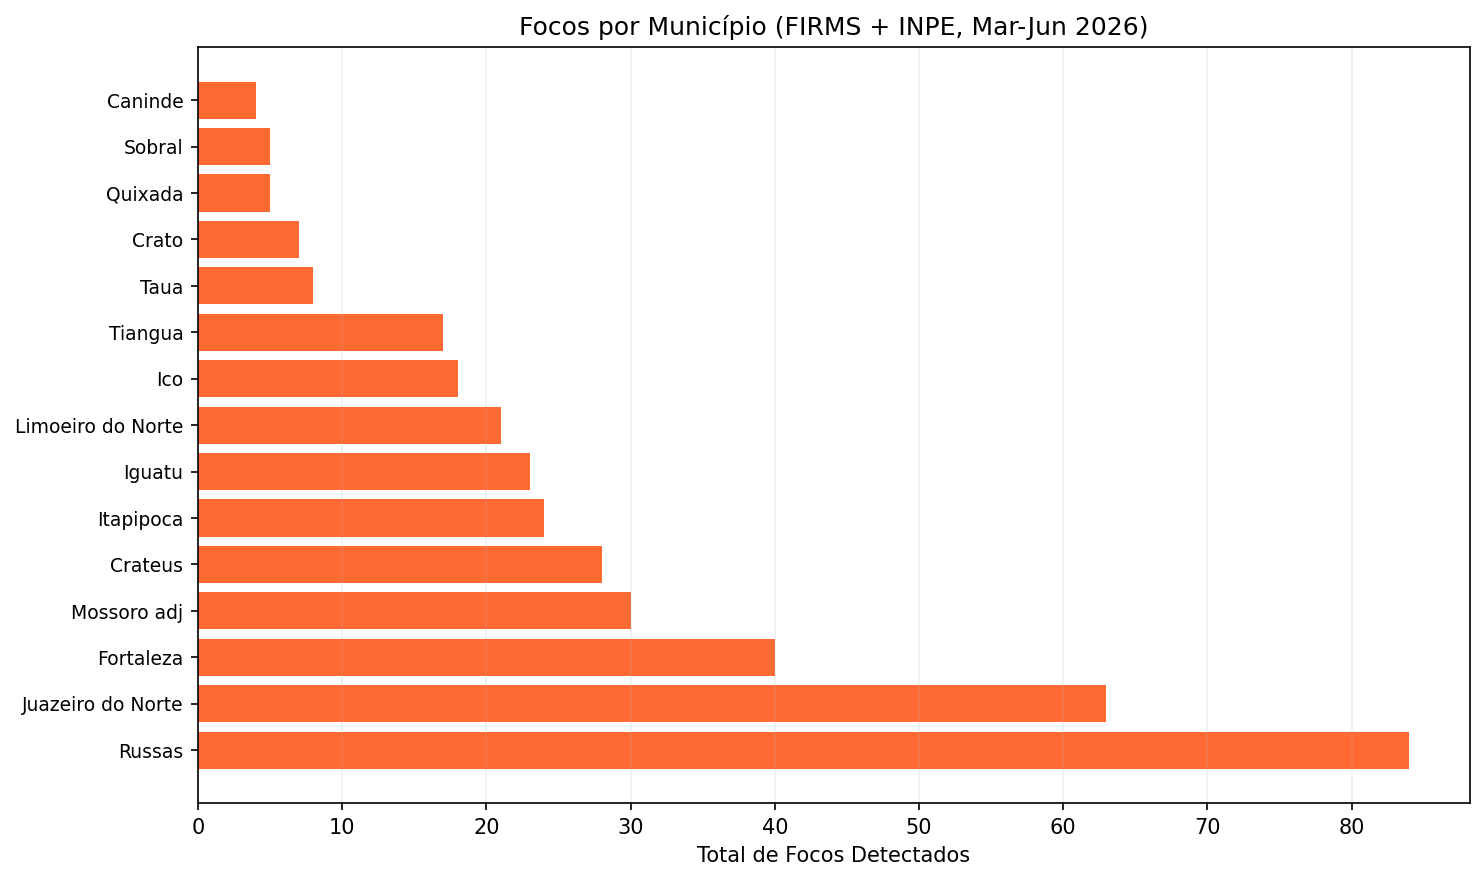
\includegraphics[width=0.75\linewidth]{figures/experimentos/05_focos_por_municipio.png}
\caption{Hotspots per monitored municipality (Exp-B real-data subset, Mar--Jun/2026).}
\label{fig:municipios-appendix}
\end{figure}

Table~\ref{tab:exp-v1} records the initial synthetic benchmark where KL-regularized Koopman-VAE underperformed shallow baselines. Table~\ref{tab:exp-v4} shows that feature expansion degraded MLP performance under data scarcity (62--67 training samples).

\begin{resulttable}{Exp-B v1: synthetic regression (200 steps, 20 nodes).}{tab:exp-v1}
\begin{tabular}{@{}lcccc@{}}
\toprule
\textbf{Model} & \textbf{RMSE}$\downarrow$ & \textbf{R\textsuperscript{2}}$\uparrow$ & \textbf{F1} & \textbf{Recall} \\
\midrule
MLP & \textbf{0.083} & \textbf{0.932} & 0.957 & 0.941 \\
XGBoost & 0.085 & 0.929 & \textbf{0.958} & 0.945 \\
Koopman-VAE (ours) & 0.260 & 0.343 & 0.828 & 0.989 \\
NeKo-PIGNN (ours) & 0.272 & 0.276 & 0.830 & 0.989 \\
\bottomrule
\end{tabular}
\end{resulttable}

\begin{resulttable}{Exp-B v4: real-data regression with feature-engineering variants.}{tab:exp-v4}
\begin{tabular}{@{}lcccc@{}}
\toprule
\textbf{Model} & \textbf{RMSE}$\downarrow$ & \textbf{R\textsuperscript{2}}$\uparrow$ & \textbf{F1} & \textbf{Precision} \\
\midrule
MLP plain & \textbf{0.143} & \textbf{0.782} & 0.936 & 0.911 \\
XGBoost + FeatEng & 0.149 & 0.767 & 0.935 & 0.902 \\
Ensemble (NeKo+XGB) & 0.149 & 0.766 & 0.930 & 0.896 \\
NeKo-PIGNN v3 & 0.173 & 0.686 & 0.906 & 0.907 \\
MLP + FeatEng + LB7 & 0.276 & 0.197 & 0.830 & 0.936 \\
\bottomrule
\end{tabular}
\end{resulttable}

Tables~\ref{tab:exp-v5}--\ref{tab:exp-v7} trace the rare-event detection iteration: v5 introduces Average Precision optimization; v6 adds focal loss and conservative XGBoost; v7 incorporates the persistence prior that raised precision to 47.5\% with only 21 false positives.

\begin{resulttable}{Exp-B v5: rare-event detection --- Average Precision and threshold metrics.}{tab:exp-v5}
\begin{tabular}{@{}lccccc@{}}
\toprule
\textbf{Model} & \textbf{AP}$\uparrow$ & \textbf{F1@best} & \textbf{Prec.} & \textbf{Recall} & \textbf{FP@0.3} \\
\midrule
MLP & 0.291 & 0.348 & 0.212 & 0.978 & 270 \\
NeKo-PIGNN v5 & \textbf{0.353} & 0.323 & \textbf{0.385} & 0.278 & \textbf{39} \\
XGBoost & 0.304 & 0.295 & 0.349 & 0.256 & 43 \\
Ensemble (NeKo+MLP) & \textbf{0.325} & \textbf{0.345} & 0.455 & 0.278 & --- \\
\bottomrule
\end{tabular}
\end{resulttable}

\begin{resulttable}{Exp-B v6: precision--recall operating modes.}{tab:exp-v6}
\begin{tabular}{@{}lccccc@{}}
\toprule
\textbf{Model} & \textbf{AP} & \textbf{F1@best} & \textbf{Prec.} & \textbf{Recall} & \textbf{FP@0.3} \\
\midrule
XGBoost (300 trees) & \textbf{0.322} & \textbf{0.427} & \textbf{0.335} & 0.589 & \textbf{28} \\
Ensemble (NeKo+XGB+MLP) & 0.315 & 0.353 & 0.217 & \textbf{0.956} & 67 \\
NeKo-PIGNN (5-seed avg.) & 0.280 & 0.324 & 0.233 & 0.533 & 81 \\
MLP (5-seed) & 0.276 & 0.350 & 0.213 & 0.989 & 282 \\
\bottomrule
\end{tabular}
\end{resulttable}

\begin{resulttable}{Exp-B v7: persistence prior combined with ML ensemble.}{tab:exp-v7}
\begin{tabular}{@{}lcccc@{}}
\toprule
\textbf{Model} & \textbf{Precision} & \textbf{Recall} & \textbf{F1} & \textbf{FP} \\
\midrule
Persistence only & 45.1\% & 48.7\% & 0.469 & 45 \\
Ensemble $\times$ Persistence & \textbf{47.5\%} & 21.1\% & 0.292 & \textbf{21} \\
NeKo $\times$ Persistence & 40.7\% & 24.4\% & 0.306 & 32 \\
XGBoost raw & 33.5\% & 58.9\% & 0.427 & 105 \\
\bottomrule
\end{tabular}
\end{resulttable}

Table~\ref{tab:three-class-full} reports per-class precision/recall/F1 from argmax classification; operational YES alerts use $P(\text{YES})\geq 0.30$ instead (Section~\ref{sec:three-level}). Table~\ref{tab:ablation-neko} confirms synergistic Koopman--PI-GNN coupling (full F1 = 0.914 vs.\ Koopman-only 0.820).

\begin{resulttable}{Full three-class classification report (Exp-B v9, XGBoost, 420 samples).}{tab:three-class-full}
\begin{tabular}{@{}lcccc@{}}
\toprule
\textbf{Class} & \textbf{Precision} & \textbf{Recall} & \textbf{F1} & \textbf{Support} \\
\midrule
NO & 0.693 & 0.973 & 0.810 & 186 \\
UNCERTAIN & 0.669 & 0.674 & 0.671 & 144 \\
YES & 0.500 & 0.078 & 0.135 & 90 \\
\midrule
Macro avg & 0.621 & 0.575 & 0.539 & 420 \\
Weighted avg & 0.644 & 0.679 & 0.618 & 420 \\
\bottomrule
\multicolumn{5}{@{}l@{}}{\textit{Note:} Operational YES alerts use $P(\text{YES})\geq 0.3$ (82.1\% precision), not argmax class.} \\
\end{tabular}
\end{resulttable}

\begin{resulttable}{NeKo-PIGNN component ablation on synthetic Rothermel propagation data.}{tab:ablation-neko}
\begin{tabular}{@{}lcccc@{}}
\toprule
\textbf{Model} & \textbf{F1} & \textbf{IoU} & \textbf{RMSE} & \textbf{R\textsuperscript{2}} \\
\midrule
NeKo-PIGNN (full) & 0.9140 & 0.8418 & 0.1083 & 0.8102 \\
Koopman-only & 0.8200 & 0.6949 & 0.1531 & 0.6215 \\
PI-GNN-only & 0.7900 & 0.6529 & 0.1682 & 0.5394 \\
Pure GNN & 0.3678 & 0.2255 & 0.2851 & $-0.32$ \\
CNN U-Net & 0.4599 & 0.2990 & 0.2514 & $-0.03$ \\
\bottomrule
\end{tabular}
\end{resulttable}


%% ===================================================================
%% Referências
%% ===================================================================

\begin{thebibliography}{99}

\bibitem{article:alencar2020}
A.~Alencar, V.~Arruda, L.~Silva, \emph{et al.}, ``Amazonia on fire: A satellite-based assessment of fires during the 2019 drought,'' \textit{Environmental Research Letters}, vol.~15, no.~3, 2020.

\bibitem{master:silva2021}
J.~Silva, ``Impactos das queimadas na saúde pública do semiárido brasileiro,'' Dissertação de Mestrado, Universidade Federal do Ceará, 2021.

\bibitem{techreport:funceme2024}
FUNCEME, ``Boletim de monitoramento de seca --- Ceará 2024,'' Relatório Técnico, 2024.

\bibitem{manual:firms2024}
NASA FIRMS, ``Fire Information for Resource Management System --- User Guide,'' 2024. [Online]. Available: \url{https://firms.modaps.eosdis.nasa.gov/}

\bibitem{article:react2023}
S.~Yao, J.~Zhao, D.~Yu, \emph{et al.}, ``ReAct: Synergizing Reasoning and Acting in Language Models,'' in \textit{Proc. ICLR}, 2023.

\bibitem{manual:langgraph2024}
LangChain, ``LangGraph Documentation,'' 2024. [Online]. Available: \url{https://langchain-ai.github.io/langgraph/}

\bibitem{article:inpe2023}
INPE, ``Banco de Dados de Queimadas --- Metodologia e Dados,'' 2023. [Online]. Available: \url{https://queimadas.dgi.inpe.br/}

\bibitem{techreport:goes2022}
NOAA, ``GOES-16 ABI L2+ Fire Detection and Characterization,'' Technical Report, 2022.

\bibitem{article:faiss2017}
J.~Johnson, M.~Douze, H.~Jégou, ``Billion-scale similarity search with GPUs,'' \textit{IEEE Trans. Big Data}, vol.~7, no.~3, 2017.

\bibitem{model:bge2024}
BAAI, ``BGE Small Embedding Model v1.5,'' 2024. [Online]. Available: \url{https://huggingface.co/BAAI/bge-small-en-v1.5}

\bibitem{article:koopman1931}
B.~O.~Koopman, ``Hamiltonian systems and transformation in Hilbert space,'' \textit{Proc. Natl. Acad. Sci.}, vol.~17, no.~5, pp.~315--318, 1931.

\bibitem{article:rothermel1972}
R.~C.~Rothermel, ``A mathematical model for predicting fire spread in wildland fuels,'' USDA Forest Service, Research Paper INT-115, 1972.

\bibitem{article:pyg2019}
M.~Fey and J.~E.~Lenssen, ``Fast graph representation learning with PyTorch Geometric,'' in \textit{Proc. ICLR Workshop on Representation Learning on Graphs and Manifolds}, 2019.

\bibitem{article:albini1976}
F.~A.~Albini, ``Estimating wildfire behavior and effects,'' USDA Forest Service, General Technical Report INT-30, 1976.

\bibitem{article:andrews2014}
P.~L.~Andrews, ``Current status and future needs of the BehavePlus Fire Modeling System,'' \textit{International Journal of Wildland Fire}, vol.~23, no.~1, pp.~21--33, 2014.

\bibitem{article:scott2001}
J.~H.~Scott and R.~E.~Burgan, ``Standard fire behavior fuel models: an extensive set for use with Rothermel's surface fire spread model,'' USDA Forest Service, Gen. Tech. Rep. RMRS-GTR-153, 2005.

\bibitem{article:finney2011}
M.~A.~Finney, I.~C.~Grenfell, C.~W.~McHugh, \emph{et al.}, ``A method for ensemble wildland fire simulation,'' \textit{Environmental Modeling \& Assessment}, vol.~16, no.~2, pp.~153--167, 2011.

\bibitem{article:raissi2019}
M.~Raissi, P.~Perdikaris, and G.~E.~Karniadakis, ``Physics-informed neural networks: A deep learning framework for solving forward and inverse problems involving nonlinear partial differential equations,'' \textit{Journal of Computational Physics}, vol.~378, pp.~686--707, 2019.

\bibitem{article:brunton2021}
S.~L.~Brunton, M.~Budisic, E.~Kaiser, and J.~N.~Kutz, ``Modern Koopman Theory for dynamical systems,'' \textit{SIAM Review}, vol.~63, no.~2, pp.~229--340, 2021.

\bibitem{article:williams2015}
M.~O.~Williams, I.~G.~Kevrekidis, and C.~W.~Rowley, ``A data--driven approximation of the Koopman operator: extending dynamic mode decomposition,'' \textit{Journal of Nonlinear Science}, vol.~25, no.~6, pp.~1307--1346, 2015.

\bibitem{article:schmid2010}
P.~Schmid, ``Dynamic mode decomposition of numerical and experimental data,'' \textit{Journal of Fluid Mechanics}, vol.~656, pp.~5--28, 2010.

\bibitem{article:kutz2016}
J.~N.~Kutz, S.~L.~Brunton, B.~W.~Brunton, and J.~L.~Proctor, ``Dynamic Mode Decomposition: Data-Driven Modeling of Complex Systems,'' SIAM, 2016.

\bibitem{article:gigante2025}
G.~Gigante, M.~Gualtieri, L.~Lauriola, and F.~Aiolli, ``Physics-Informed Graph Neural Networks: A Systematic Survey,'' \textit{arXiv preprint}, arXiv:2503.11209, 2025.

\bibitem{article:gao2023}
Z.~Gao, T.~Yan, and H.~Hu, ``Physics-informed graph neural networks for predicting wildfire spread,'' in \textit{Proc. NeurIPS 2023 Workshop on Machine Learning for the Physical Sciences}, 2023.

\bibitem{article:li2025}
S.~Li, Y.~Wang, and S.~Pai, ``A physics-informed graph neural network approach for wildfire spread forecasting,'' \textit{Environmental Modelling \& Software}, vol.~186, p.~106315, 2025.

\bibitem{article:hodzic2024}
E.~Hodzic, A.~R.~F.~O.~P., and J.~Davila, ``Fire Risk Prediction based on Satellite Data and Machine Learning: A Systematic Literature Review,'' \textit{IEEE Access}, vol.~12, pp.~106557--106583, 2024.

\bibitem{article:gargiulo2023}
F.~Gargiulo, D.~G.~Marino, A.~Zinno, \emph{et al.}, ``A multi-source satellite data approach for wildfire detection and monitoring,'' \textit{Remote Sensing}, vol.~15, no.~8, p.~1987, 2023.

\bibitem{article:giglio2016}
L.~Giglio, W.~Schroeder, and C.~O.~Justice, ``The Collection~6 MODIS active fire detection algorithm and fire products,'' \textit{Remote Sensing of Environment}, vol.~178, pp.~31--41, 2016.

\bibitem{article:schroeder2014}
W.~Schroeder, P.~Olszewski, and J.~T.~Morisette, ``The New VIIRS~375~m active fire detection data product: Algorithm description and initial assessment,'' \textit{Remote Sensing of Environment}, vol.~143, pp.~85--96, 2014.

\bibitem{article:wooster2021}
M.~J.~Wooster, G.~J.~Roberts, L.~Giglio, \emph{et al.}, ``Satellite remote sensing of active fires: History and current status, applications and future requirements,'' \textit{Remote Sensing of Environment}, vol.~267, p.~112694, 2021.

\bibitem{article:mccarty2024}
J.~L.~McCarty, J.~V.~A.~Smith, and D.~P.~Roy, ``Trends in fire activity and associated emissions in South America from 2003 to 2023,'' \textit{Global Change Biology}, vol.~30, no.~4, p.~e17243, 2024.

\bibitem{article:alves2023}
D.~B.~Alves, F.~J.~S.~Moreira, and R.~L.~S.~Souza, ``Machine learning for wildfire prediction in the Brazilian Cerrado and Caatinga biomes,'' \textit{Ecological Informatics}, vol.~78, p.~102362, 2023.

\bibitem{article:arruda2025}
V.~S.~Arruda, A.~P.~M.~Ramos, and C.~H.~L.~Silva Jr., ``Deep learning approaches for burned area mapping in the Amazon and Caatinga biomes using Sentinel-2 imagery,'' \textit{ISPRS Journal of Photogrammetry and Remote Sensing}, vol.~219, pp.~245--261, 2025.

\bibitem{article:vaswani2017}
A.~Vaswani, N.~Shazeer, N.~Parmar, \emph{et al.}, ``Attention is all you need,'' in \textit{Proc. NeurIPS}, 2017.

\bibitem{article:brown2020}
T.~B.~Brown, B.~Mann, N.~Ryder, \emph{et al.}, ``Language models are few-shot learners,'' in \textit{Proc. NeurIPS}, 2020.

\bibitem{article:wei2022}
J.~Wei, X.~Wang, D.~Schuurmans, \emph{et al.}, ``Chain-of-thought prompting elicits reasoning in large language models,'' in \textit{Proc. NeurIPS}, 2022.

\bibitem{article:lewis2020}
P.~Lewis, E.~Perez, A.~Piktus, \emph{et al.}, ``Retrieval-augmented generation for knowledge-intensive NLP tasks,'' in \textit{Proc. NeurIPS}, 2020.

\bibitem{article:izacard2022}
G.~Izacard, P.~Lewis, M.~Lomeli, \emph{et al.}, ``Atlas: Few-shot learning with retrieval augmented language models,'' \textit{Journal of Machine Learning Research}, vol.~24, pp.~1--43, 2022.

\bibitem{article:xu2019}
K.~Xu, W.~Hu, J.~Leskovec, and S.~Jegelka, ``How powerful are graph neural networks?'' in \textit{Proc. ICLR}, 2019.

\bibitem{article:hamilton2017}
W.~Hamilton, Z.~Ying, and J.~Leskovec, ``Inductive representation learning on large graphs,'' in \textit{Proc. NeurIPS}, 2017.

\bibitem{article:velickovic2018}
P.~Velickovic, G.~Cucurull, A.~Casanova, \emph{et al.}, ``Graph attention networks,'' in \textit{Proc. ICLR}, 2018.

\bibitem{article:deepseek2025}
DeepSeek-AI, ``DeepSeek-R1: Incentivizing Reasoning Capability in LLMs via Reinforcement Learning,'' \textit{arXiv preprint}, arXiv:2501.12948, 2025.

% ---- FIM DAS NOVAS REFERÊNCIAS (v3.2) ----

% ===== NOVAS REFERÊNCIAS: LITERATURE EXPANSION (Jun/2026) =====
% Digital Twins, Koopman, PINNs, LangGraph/Agentic AI

%%% DIGITAL TWINS %%%
\bibitem{article:grieves2014}
M.~Grieves, ``Digital Twin: Manufacturing Excellence through Virtual Factory Replication,'' White Paper, Florida Institute of Technology, 2014.

\bibitem{article:tao2019}
F.~Tao, H.~Zhang, A.~Liu, and A.~Y.~C.~Nee, ``Digital Twin in Industry: State-of-the-Art,'' \textit{IEEE Trans. Ind. Inform.}, vol.~15, no.~4, pp.~2405--2415, 2019.

\bibitem{article:barricelli2019}
B.~R.~Barricelli, E.~Casiraghi, and D.~Fogli, ``A survey on Digital Twin: Definitions, characteristics, applications, and design implications,'' \textit{IEEE Access}, vol.~7, pp.~167653--167671, 2019.

\bibitem{article:rasheed2020}
A.~Rasheed, O.~San, and T.~Kvamsdal, ``Digital Twin: Values, challenges and enablers from a modeling perspective,'' \textit{IEEE Access}, vol.~8, pp.~21980--22012, 2020.

\bibitem{article:fuller2020}
A.~Fuller, Z.~Fan, C.~Day, and C.~Barlow, ``Digital Twin: Enabling technologies, challenges and open research,'' \textit{IEEE Access}, vol.~8, pp.~108952--108971, 2020.

\bibitem{article:jones2020}
D.~Jones, C.~Snider, A.~Nassehi, J.~Yon, and B.~Hicks, ``Characterising the Digital Twin: A systematic literature review,'' \textit{CIRP J. Manuf. Sci. Technol.}, vol.~29, pp.~36--52, 2020.

\bibitem{article:bauer2021nature}
P.~Bauer, P.~D.~Dueben, T.~Hoefler, \textit{et al.}, ``The Digital Twin of the Earth System,'' \textit{Nature Computational Science}, vol.~1, no.~10, pp.~654--656, 2021.

\bibitem{article:voosen2020}
P.~Voosen, ``Europe builds `digital twin' of Earth to hone climate forecasts,'' \textit{Science}, vol.~370, no.~6513, p.~158, 2020.

\bibitem{article:nativi2021}
S.~Nativi, P.~Mazzetti, M.~Santoro, \textit{et al.}, ``Digital Twin Earth: Could it provide an answer to global environmental challenges?'' \textit{Environmental Science \& Policy}, vol.~126, pp.~10--18, 2021.

\bibitem{article:bauer2023natrev}
P.~Bauer, T.~Quintino, N.~Wedi, \textit{et al.}, ``Earth System Digital Twins: A new paradigm for environmental science,'' \textit{Nature Reviews Earth \& Environment}, vol.~4, no.~8, pp.~545--558, 2023.

%%% KOOPMAN OPERATOR THEORY %%%
\bibitem{article:mezic2013}
I.~Mezi\'{c}, ``Analysis of fluid flows via spectral properties of the Koopman Operator,'' \textit{Annual Review of Fluid Mechanics}, vol.~45, pp.~357--378, 2013.

\bibitem{article:rowley2009}
C.~W.~Rowley, I.~Mezi\'{c}, S.~Bagheri, P.~Schlatter, and D.~S.~Henningson, ``Spectral analysis of nonlinear flows,'' \textit{Journal of Fluid Mechanics}, vol.~641, pp.~115--127, 2009.

\bibitem{article:brunton2016sindy}
S.~L.~Brunton, J.~L.~Proctor, and J.~N.~Kutz, ``Discovering governing equations from data by sparse identification of nonlinear dynamical systems,'' \textit{Proc. Natl. Acad. Sci.}, vol.~113, no.~15, pp.~3932--3937, 2016.

\bibitem{article:lusch2018}
B.~Lusch, J.~N.~Kutz, and S.~L.~Brunton, ``Deep learning for universal linear embeddings of nonlinear dynamics,'' in \textit{Proc. NeurIPS}, vol.~31, 2018.

\bibitem{article:bengio2009curriculum}
Y.~Bengio, J.~Louradour, R.~Collobert, and J.~Weston, ``Curriculum learning,'' in \textit{Proc. 26th International Conference on Machine Learning (ICML)}, pp.~41--48, 2009.

\bibitem{article:takeishi2017}
N.~Takeishi, Y.~Kawahara, and T.~Yairi, ``Learning Koopman invariant subspaces for Dynamic Mode Decomposition,'' in \textit{Proc. NeurIPS}, vol.~30, 2017.

\bibitem{article:proctor2016}
J.~L.~Proctor, S.~L.~Brunton, and J.~N.~Kutz, ``Dynamic Mode Decomposition with control,'' \textit{SIAM J. Appl. Dyn. Syst.}, vol.~15, no.~1, pp.~142--161, 2016.

\bibitem{article:baddoo2023}
P.~J.~Baddoo, B.~Herrmann, B.~J.~McKeon, J.~N.~Kutz, and S.~L.~Brunton, ``Physics-Informed Dynamic Mode Decomposition,'' \textit{Proc. R. Soc. A}, vol.~479, no.~2271, p.~20220576, 2023.

\bibitem{article:morton2019}
J.~Morton, F.~D.~Witherden, A.~Jameson, and M.~J.~Kochenderfer, ``Deep dynamical modeling and control of unsteady fluid flows,'' \textit{Neural Computation}, vol.~31, no.~12, pp.~2469--2501, 2019.

%%% PHYSICS-INFORMED NEURAL NETWORKS %%%
\bibitem{article:karniadakis2021}
G.~E.~Karniadakis, I.~G.~Kevrekidis, L.~Lu, \textit{et al.}, ``Physics-informed machine learning,'' \textit{Nature Reviews Physics}, vol.~3, no.~6, pp.~422--440, 2021.

\bibitem{article:lu2021deepxde}
L.~Lu, X.~Meng, Z.~Mao, and G.~E.~Karniadakis, ``DeepXDE: A deep learning library for solving differential equations,'' \textit{SIAM Review}, vol.~63, no.~1, pp.~208--228, 2021.

\bibitem{article:cuomo2022}
S.~Cuomo, V.~S.~Di~Cola, F.~Giampaolo, \textit{et al.}, ``Scientific machine learning through physics-informed neural networks: Where we are and what's next,'' \textit{J. Sci. Comput.}, vol.~92, no.~3, p.~88, 2022.

\bibitem{article:mao2024pinn}
Z.~Mao, Y.~Yu, G.~E.~Karniadakis, and L.~Lu, ``Physics-informed neural networks for wildfire spread simulation,'' \textit{J. Comput. Phys.}, vol.~507, p.~112978, 2024.

\bibitem{article:xi2023}
Z.~Xi, W.~Chen, X.~Guo, \textit{et al.}, ``The rise and potential of large language model based agents: A survey,'' arXiv preprint arXiv:2309.07864, 2023.

\bibitem{article:wang2024survey}
L.~Wang, C.~Ma, X.~Feng, \textit{et al.}, ``A survey on large language model based autonomous agents,'' \textit{Frontiers of Computer Science}, vol.~18, no.~6, p.~186345, 2024.

\bibitem{article:park2023}
J.~S.~Park, J.~C.~O'Brien, C.~J.~Cai, \textit{et al.}, ``Generative agents: Interactive simulacra of human behavior,'' in \textit{Proc. ACM UIST}, 2023.

\bibitem{article:shinn2023}
N.~Shinn, F.~Cassano, A.~Gopinath, K.~Narasimhan, and S.~Yao, ``Reflexion: An autonomous agent with dynamic memory and self-reflection,'' in \textit{Proc. NeurIPS}, vol.~36, 2023.

\bibitem{article:schick2023}
T.~Schick, J.~Dwivedi-Yu, R.~Dess\`{i}, \textit{et al.}, ``Toolformer: Language models can teach themselves to use tools,'' in \textit{Proc. NeurIPS}, vol.~36, 2023.

\bibitem{article:patil2023}
S.~G.~Patil, T.~Zhang, X.~Wang, and J.~E.~Gonzalez, ``Gorilla: Large language model connected with massive APIs,'' in \textit{Proc. NeurIPS}, vol.~36, 2023.

\bibitem{article:gao2024rag}
Y.~Gao, Y.~Xiong, X.~Gao, \textit{et al.}, ``Retrieval-Augmented Generation for large language models: A survey,'' arXiv preprint arXiv:2312.10997, 2024.

% --- FIM DAS NOVAS REFERÊNCIAS ---

%%% KEY RECENT DIGITAL TWIN FIRE PAPERS %%%
\bibitem{article:morsali2026}
M.~Morsali and S.~H.~Khajavi, ``Digital Twin and Agentic AI for Wild Fire Disaster Management: Intelligent Virtual Situation Room (IVSR),'' \textit{arXiv preprint}, arXiv:2602.08949, 2026.

\bibitem{article:webb2026}
C.~Webb, M.~Habibpour, M.~H.~Raha, \emph{et al.}, ``FIRE-VLM: A Vision-Language-Driven Reinforcement Learning Framework for UAV Wildfire Tracking in a Physics-Grounded Fire Digital Twin,'' \textit{arXiv preprint}, arXiv:2601.03449, 2026.

\bibitem{article:raha2025}
M.~H.~Raha, A.~R.~Tavakkoli, C.~Webb, \emph{et al.}, ``FIRETWIN: Digital Twin Advancing Multi-Modal Sensing, Interactive Analytics for Wildfire Response,'' \textit{arXiv preprint}, arXiv:2510.18879, 2025.

\bibitem{article:esparza2025}
I.~Esparza, A.~Battal, and A.~Mostafavi, ``GraphFire-X: Physics-Informed Graph Attention Networks for Building-Scale Wildfire Preparedness,'' \textit{arXiv preprint}, arXiv:2512.20813, 2025.

\bibitem{article:michail2025}
D.~Michail, I.~Davalas, \emph{et al.}, ``FireCastNet: Earth-as-a-Graph for Seasonal Fire Prediction,'' \textit{arXiv preprint}, arXiv:2502.01550, 2025 (v2).

% --- REFERÊNCIAS ADICIONADAS (TASK-116, jun/2026) ---

\bibitem{article:vogiatzoglou2024}
K.~Vogiatzoglou, C.~Papadimitriou, V.~Bontozoglou, and K.~Ampountolas, ``Physics-informed neural networks for parameter learning of wildfire spreading,'' \textit{arXiv preprint}, arXiv:2406.14591, 2024.

\bibitem{article:aimnet2025}
Z.~Zhou, X.~Wang, Y.~Yan, \emph{et al.}, ``AIMNET: An IoT-Empowered Digital Twin for Continuous Gas Emission Monitoring and Early Hazard Detection,'' \textit{arXiv preprint}, arXiv:2512.06148. Accepted by IEEE Internet of Things Magazine, 2025.

\bibitem{article:hrdt2025}
Z.~Shen and H.~Zhou, ``Hazard-Responsive Digital Twin for Climate-Driven Urban Resilience and Equity,'' \textit{arXiv preprint}, arXiv:2510.22941, 2025.

\bibitem{website:mapbiomas}
MapBiomas, ``MapBiomas Fogo --- Coleção de Mapas Anuais de Área Queimada,'' 2024. [Online]. Available: \url{https://mapbiomas.org/}

\bibitem{article:prapas2023}
I.~Prapas, \emph{et al.}, ``Earth System Deep Learning Towards a Global Digital Twin of Wildfires,'' in \textit{EGU General Assembly}, 2023.

\end{thebibliography}

\end{document}
